%=========================================================================

%- potreba mit 10-20 vysazenych stran / 20-40 normostran
%- na jednu plne potistenou stranu se vleze 1,65 (s nadpisem chapter) nebo 2,36 (bez nadpisu) normostran

% Setting the depth of sections numbering
\setcounter{secnumdepth}{2}
% Setting the depth of sections to appear in the table of contents.
\addtocontents{toc}{\protect\setcounter{tocdepth}{1}}


%=========================================================================
%=========================================================================
\chapter{Introduction}
% 1 - 2 ns

In todays world the localization of the aerial objects is an essential component of two main domains, a public air traffic control (ATC) and a national defense. In both cases the main purpose of the system is to estimate the distance and the 3D position of a given airborne vehicle.

In case of the ATC, the airports mainly rely on the multilateration systems which specialize on surveillance and control of air traffic during all flight phases \cite{Gaviria:newStrategiesMLAT}. The design of such a system expects that the aircraft are equipped with a secondary surveillance radar transponders which periodically emit the signals to the ground receiving stations, however primary radars are widely used as well \cite{Airtrafficmuseum}. In the military segment the aerial object localization mainly serves the purpose of detecting and identifying a intruder which might pose a threat for a given area under protection. In this scenario only primary radars are used since the aerial objects are not expected to cooperate.

Even though being widely used, radar based localization systems suffer from several drawbacks. Radar is a device based on the active emission of the radio signal \cite{toomay2012radar}. In order to localize distant objects, a huge amount of energy must be radiated to make sure it would return from the target and a small amount of energy returned might be easily disrupted \cite{Airtrafficmuseum}. What is more, in defense applications it is not desirable that the tracked object would find out that it is being tracked, which is the condition an actively radiating system, such as a radar, cannot achieve. Last but not least, the professional class radars in use by both public segment and military are in general expensive, large and heavy devices not suitable for mobile deployment.

In this work, I propose a fully autonomous passive multi-camera system for detecting, tracking and localizing aerial objects which is based merely on ordinary RGB cameras --- the Optical Localization System (OLS). Since the system does not rely on active emission of a signal, but rather captures the optical information from the environment, it can be used for secret localization of aerial targets. The system is designed to be well suited for mobility and temporary deployment since each camera station used weigh no more than twenty kilograms and the whole system is relatively inexpensive as well.


%-------------------------------------------------------------------------
%-------------------------------------------------------------------------
\section{Background} \label{txt:background}

The principle of the optical localization of objects, which is based on triangulation, is well known for quite a long time. The first devices which were designed to allow an operator to estimate a distance to a given object using mechanical and optical principles --- optical range finders --- emerged in the second half of the 18th century \cite{bud1998instruments}. Ever since, the optical range finders had been mostly used for military operations in order to estimate the position of either naval, airborne or terrestrial targets until the World War II when radar was invented.

The OLS system aims to utilize the same principle as the old optical range finders. However, instead of an optical device requiring the operator to aim on the target manually the OLS takes advantage of the RGB cameras and the image processing techniques capable of detecting, tracking and localizing the target autonomously without the need for a human to interfere. Furthermore, with the use of sensors capable of finding a geographical position of each observer unit the OLS system estimates a global geographical position of a given target (not only the distance or relative position).


%-------------------------------------------------------------------------
%-------------------------------------------------------------------------
\section{Related Work}
% 1 - 2 ns

Professional systems aiming on automatic localization of aerial (as well as terrestrial and underwater) targets mostly rely on active devices, such as radars or sonars and there is very little use of pure passive optical devices (such as RGB cameras, thermal imaging cameras, etc.). The reason might be the complexity of the whole solution or the operation constrained by the weather conditions.

On the other hand since the application of multiple view geometry has been one of hot topics in the computer vision during the past decade, many R\&D groups (specializing mostly on robotics) attempt to base their solutions on multi-camera optical localization.

One of the widely used approaches is to set up so called \textit{intelligent space} \cite{intelligentSpace}, the bounded area under surveillance of multiple cameras reporting to the the central system. In \cite{Multi-Camera_Sensor_System_for_3D_Segmentation} multiple terrestrial robots are detected, tracked and localized by the multi-camera system. For all cameras, the intrinsics and extrinsics are known beforehand and do not change over time.  A similar approach is used also in \cite{Localization_and_Geometric_Reconstruction_of_Mobile_Robots} but this system uses the robot's odometers as well in order to improve the resulting position estimated by the optical system. The system presented in \cite{A_3D_visual_localization} then relies on four ordinary RGB cameras with known parameters (intrinsics, extrinsics) to estimate the position of the easy to detect and static object using the Perpendicular Foot Method algorithm.

Even though all of the aforementioned approaches utilize the ordinary RGB cameras for detection and tracking and in general estimate the location of the object using the triangulation algorithm, they all assume the object moves strictly within the specified bounded region and they rely on fixed positions of the cameras. Thus, they do not have to deal with the imprecisions arose from the uncertainty of the current camera pose estimation and with the problems of handing off the target to other camera units once a target moves out of the operational range of the given camera. 

As for the detection and tracking of the distant aerial targets, one of the most recent approaches was presented by Rozantsev et al. \cite{DBLP:journals/corr/RozantsevLF14}. The algorithm combines both the appearance and motion clues in order to distinguish the object from the complex background.

%-------------------------------------------------------------------------
%-------------------------------------------------------------------------
\section{Thesis Organization}

Chapter \ref{txt:system_overview} presents the general information about the system and describes its operation in a big picture. Chapter \ref{txt:camera_unit} analyzes the devices which make up a camera unit (a core hardware component of the system) and presents the corresponding model. The next Chapter~\ref{txt:stationing_and_rectification} explains the necessity of finding the precise position and orientation of the whole camera station as well as evaluating the deviations between the camera unit model and its real construction. Chapter \ref{txt:detection_and_tracking} discusses the core computer vision components of the system, the detection and tracking. Chapter \ref{txt:implementation} goes through the implementation details and the final Chapter \ref{txt:conclusion} concludes the work.


%=========================================================================
%=========================================================================
\chapter{System Overview} \label{txt:system_overview}

This section presents the main hardware building blocks of the OLS, the camera stations, and describes the basic pipeline which the system must follow in order to localize a given object. From the implementation point of view, the OLS is built on the ROS framework (see Chapter \ref{txt:implementation}) which presents certain conventions, most importantly the orientation of the coordinate frame which will be used throughout the document (see Figure \ref{fig:frame_convention}).

%% ROS frame conventions
\begin{figure}[htb]
	\centering
	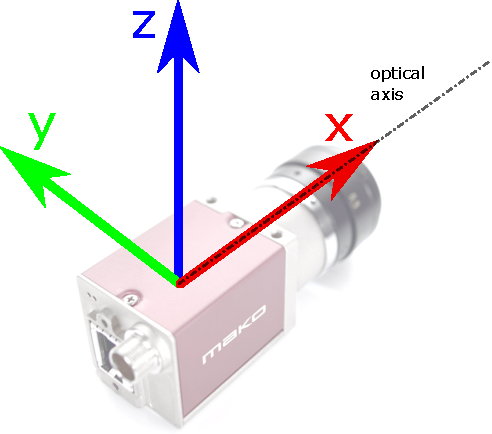
\includegraphics[width=4cm]{fig/frame_convention.pdf}
	\caption{Frame orientation convention adopted from ROS which will be used throughout the work --- a right handed coordinate system with X axis aiming forward, Y axis left and Z axis up.}
	\label{fig:frame_convention}
\end{figure}

%-------------------------------------------------------------------------
%-------------------------------------------------------------------------
\section{Principle of Object Localisation}
\todo{Obecne jak to funguje}

\begin{figure*}[t]\centering % Using \begin{figure*} makes the figure take up the entire width of the page
	\centering
	
\includegraphics[width=0.45\linewidth, height=5cm]{fig/placeholder.pdf}
	
\includegraphics[width=0.45\linewidth, height=5cm]{fig/placeholder.pdf}
	\caption{\todo{Dodat caption}}
	\label{fig:WidePicture}
\end{figure*}

\vata[4]

%-------------------------------------------------------------------------
%-------------------------------------------------------------------------
\section{System Topology}

The main building block of the OLS system is a \texttt{camera station} (CS). CS consists of the \texttt{camera unit} (CU), which is a collection of hardware necessary for capturing the images, manipulating the position of the camera and estimating the geographical coordinates of the CS (for detailed description see Chapter \ref{txt:camera_unit}), and the computation unit processing the data (a PC or other device). In general, the OLS is designed to work with an arbitrary number of CSs (of course, there must be at least two stations) and there are two types of CSs:

\paragraph{overview station} Only one of the CSs is selected to become the overview station. Its main objective is to scan the surrounding environment, discover the aerial objects, distribute the information to the tracking stations and prospectively take part in the tracking phase. The station disposes of the camera equipped with the zooming lens allowing for scanning greater distances and the PC serving the purpose of the main entry point for the human operator (see Section \ref{txt:hardware}).

\paragraph{tracking station} All other stations become tracking stations which scan the surrounding environment, detect the aerial objects and perform tracking. All cameras are equipped with fixed focal length lenses. \\

As for the network topology, the OLS is based on a star pattern where each tracking station communicates only with the overview station (see Section \ref{txt:hardware}). The positional organization of the CSs depends on the number of tracking stations, which should always be placed so that their positions projected to the horizontal plane would form a regular polygon with the overview unit in the center (see Figure \ref{fig:system_overview}), however, in more complex environments this condition does not have to strictly hold (see Figure \ref{fig:spilberk_camera_units}).

%% Schema of camera units organized in triangle.
%% Use case of camera units - placed on map of Brno's Spilberk
\begin{figure}[htb]
	\centering
	\begin{minipage}{.45\textwidth}
		\centering
		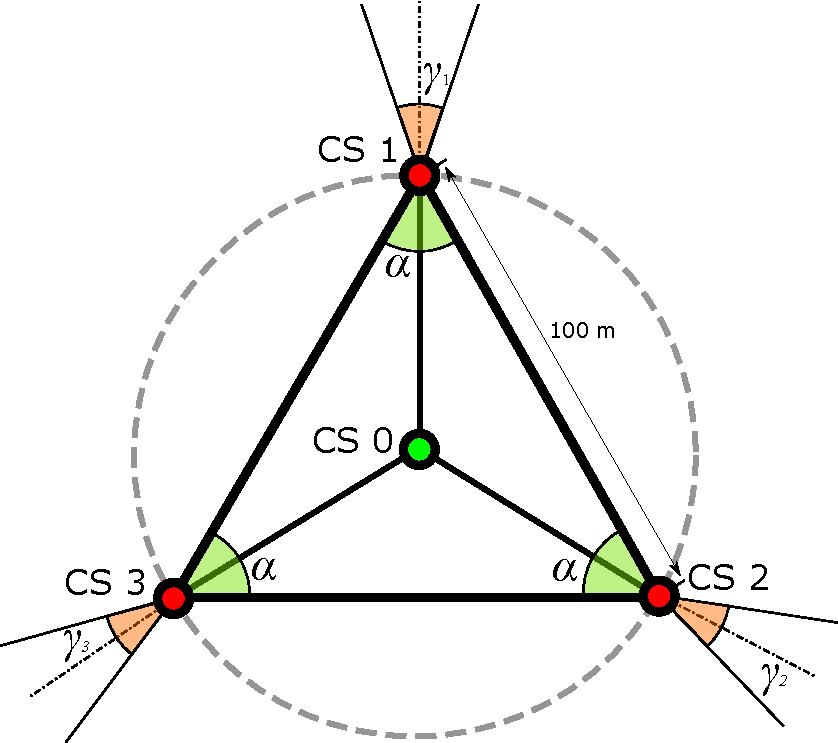
\includegraphics[width=.99\linewidth]{fig/system_overview.pdf}
		\captionof{figure}{Schematic view of the ideal-case organization of all camera units where all three tracking units make up an equilateral triangle with the overview unit in the middle. The initial orientation of the tracking units is shown as well as their FOVs $\gamma_{1-3} = 38^{\circ}$ (assuming camera Prosilica GT 1290C and a lens with equivalent 50mm focal length).}
		\label{fig:system_overview}
	\end{minipage}
	\hfill
	\begin{minipage}{.48\textwidth}
		\centering
		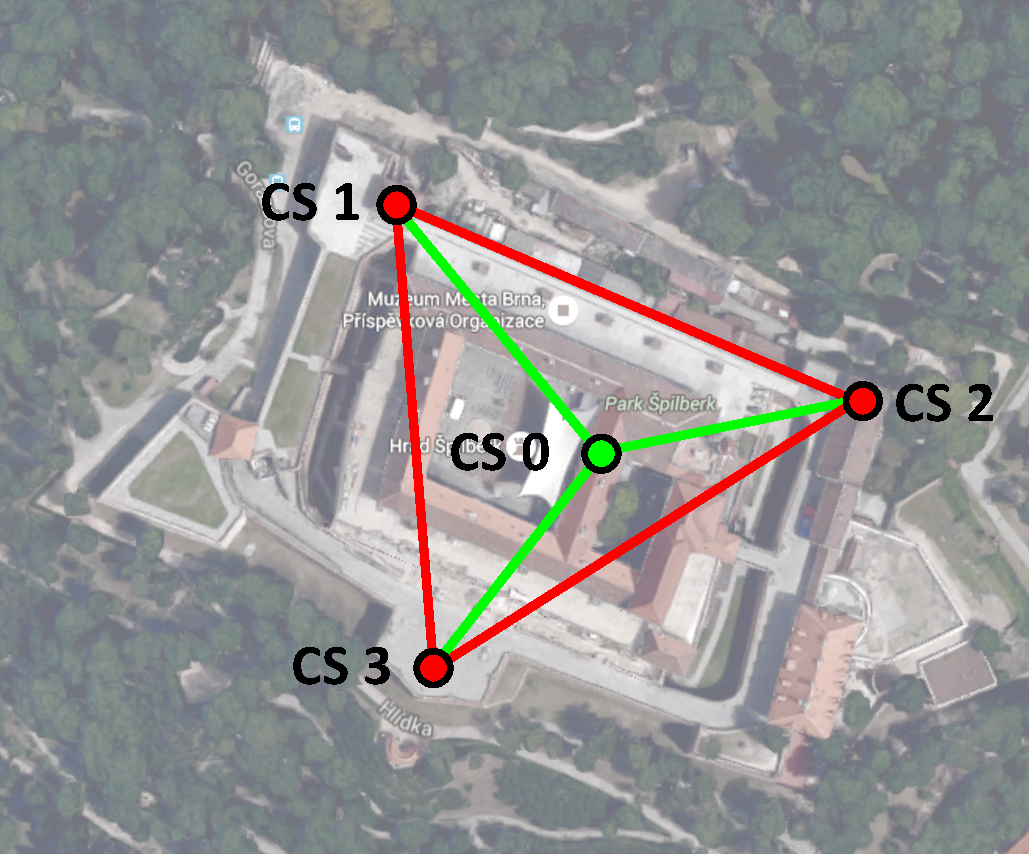
\includegraphics[width=.99\linewidth]{fig/spilberk_camera_units.pdf}
		\captionof{figure}{Use case scenario showing the organization of the camera units within the system set to protect a real world area (the castle Spilberk in Brno, Czech Republic). As can be seen in the Figure, given the possibilities of the protected area (some CUs mounted on the rooftops) the CUs do not form an equilateral triangle, neither is the overview unit positioned in the middle.}
		\label{fig:spilberk_camera_units}
	\end{minipage}
\end{figure}

%-------------------------------------------------------------------------
%-------------------------------------------------------------------------
\section{Hardware Architecture}

Considering the big picture of the system, OLS consists of four camera stations, a hardware devices necessary for network communication and the peripherals for manual control. There are two types of camera stations, a tracking station and an overview station (see Section~\ref{txt:system_overview}). All stations communicate with each other vie Ethernet switch. The peripheral devices (keyboard, joystick) allowing the operator to manually control the system are connected to the overview station (see Figure \ref{fig:hw_ols}).

%% The big picture diagram of the hardware components of the OLS
\begin{figure}[htb]
	\centering
	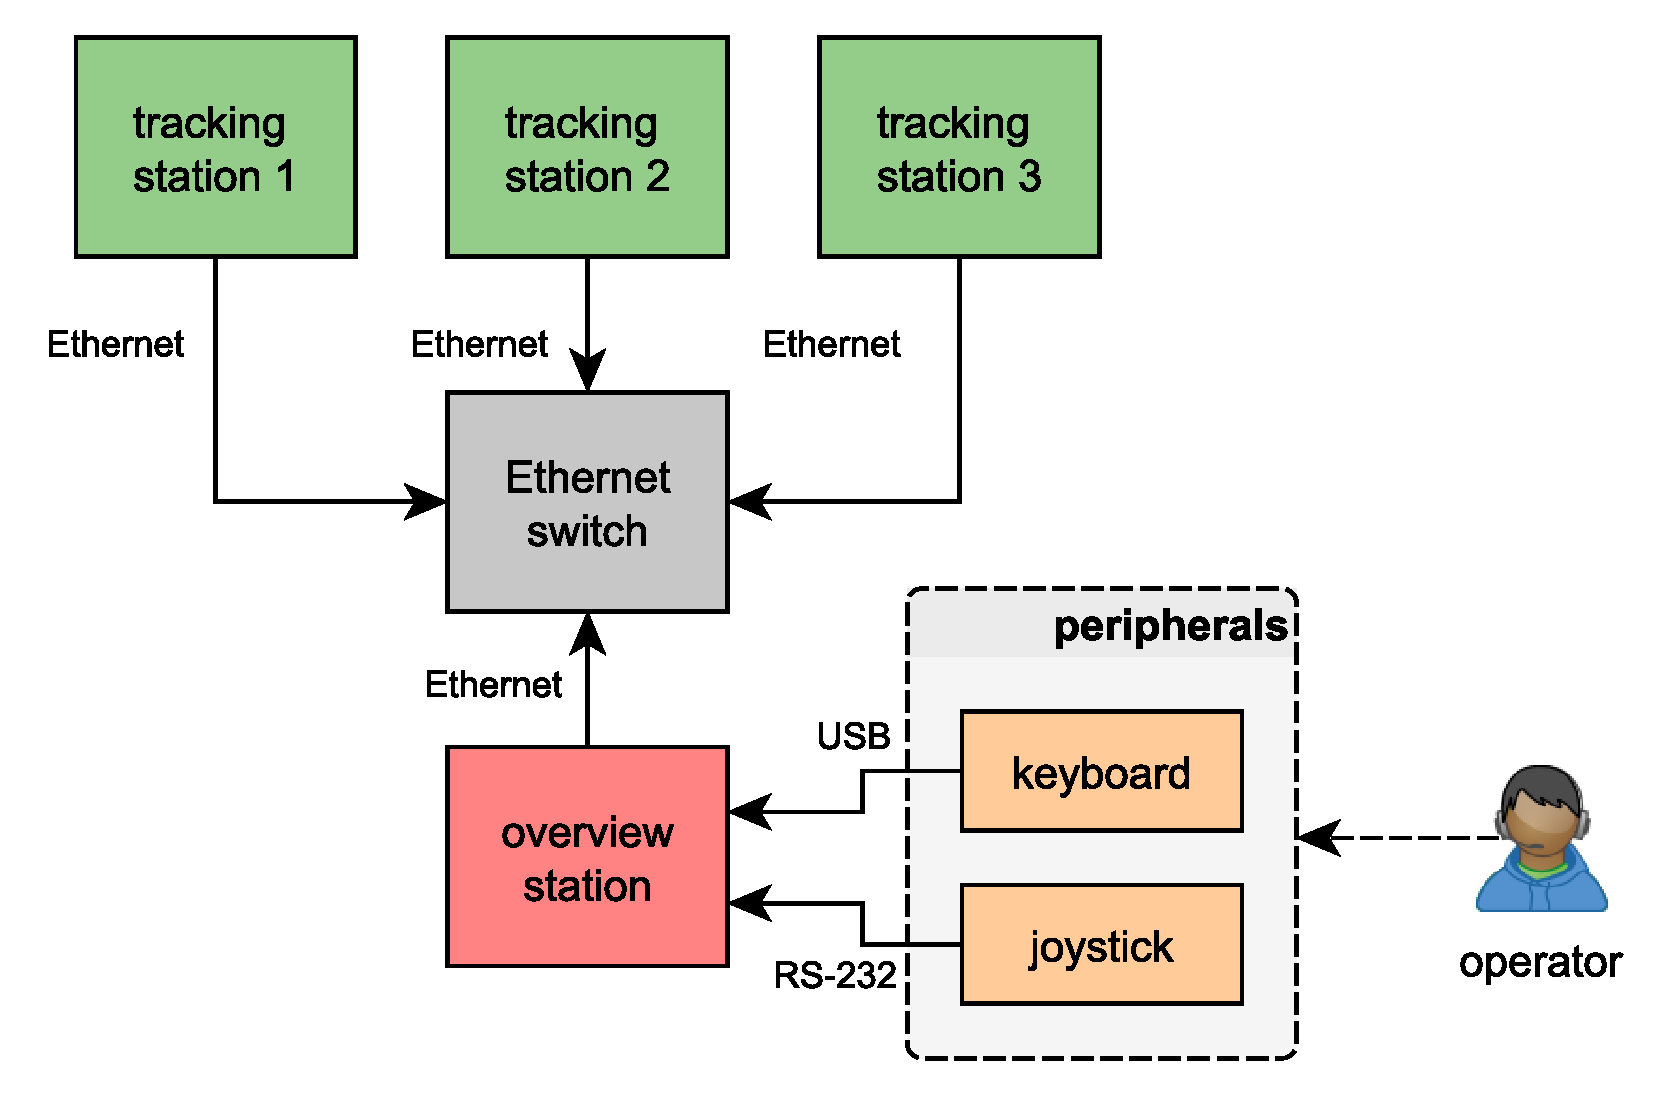
\includegraphics[width=9cm]{fig/hw_ols.pdf}
	\caption{The big picture diagram of the main components of the OLS.}
	\label{fig:hw_ols}
\end{figure}

A camera station itself consists of a camera unit (see Section \ref{txt:camera_unit}) and a computer running the OLS software. The camera unit is controlled by the controller \texttt{STM32F4007} which communicates with the manipulator \texttt{Flir PTU D46-70}, a GPS module and a zoom lens. The camera \texttt{Prosilica GT 1290C} is connected directly to a computer running OLS system (for more details see Figure \ref{fig:hw_camera_unit}).

%% The diagram of the hardware components of the camera unit
\begin{figure}[htb]
	\centering
	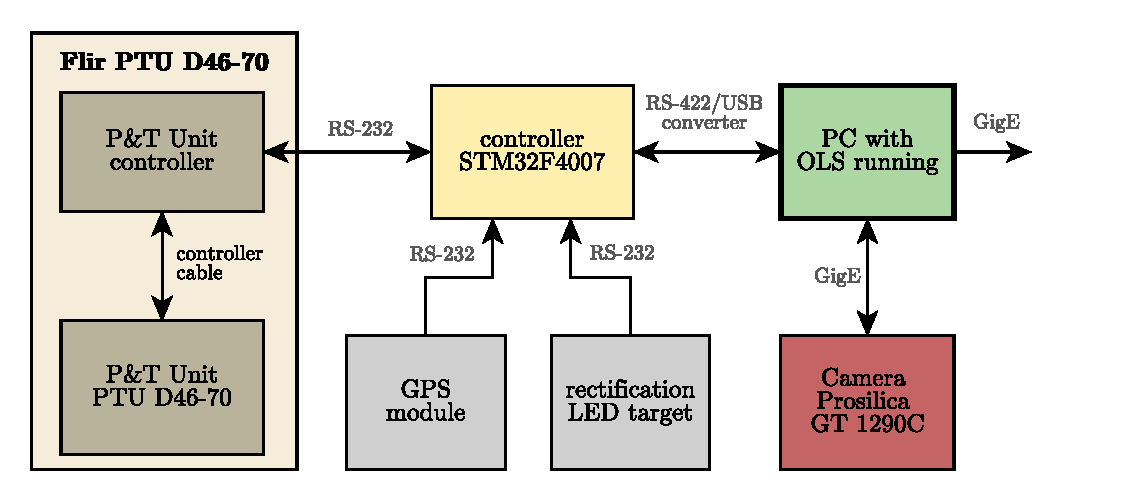
\includegraphics[width=9cm]{fig/hw_camera_unit.pdf}
	\caption{The diagram of the hardware components of the camera unit depicting both the hardware devices and the communication standards.}
	\label{fig:hw_camera_unit}
\end{figure}

%-------------------------------------------------------------------------
%-------------------------------------------------------------------------
\section{Software Architecture}

Before the 3D location of the given target is estimated, the system must perform several operations. After powering on the system all camera stations start scanning the surrounding environment. The scanning process is autonomous, however, should the operator decide to interfere, the overview unit is used in order to control the camera (through the GUI and peripheral devices). 

Once any of the stations detects an aerial object, it saves the visual information distinguishing the object and notifies the overview station. The overview station selects the best candidate(s) to track the newly discovered object and notifies the chosen unit with the essential data about the object (direction in which it was spotted, visual clues, global id, etc.).

The other unit(s) must first detect the newly spotted object. If it succeeds it initiates the tracking. The overview unit then computes the triangulation and estimates the 3D location of the target.

%=========================================================================
%=========================================================================
\chapter{Localisation Precision Analysis}
\todo{Rozdelit typy chyb}
\todo{Error map - zavislost chyby lokalizace na vrcholovem uhlu a velikosti baze a poctu jednotek}
\todo{Zavislost presnosti na chybe trackeru v px - v simulatoru}

\vata[20]

%=========================================================================
%=========================================================================
%\chapter{Sensitivity analysis} \label{txt:sensitivity_analysis}
%The precision of the system can be defined in the means of the frame-by-frame Euclidean distance between the estimated location and the real (ground truth) location of the given target. The precision is impacted by multiple independent factors, thus it is essential to perform the sensitivity analysis in order to discover and prospectively alleviate the most prominent contributors of the overall error. 
%
%- vysvetleni typu chyb:
%	- system error (systemova chyba)
%		- nesoulad modelu CU s realnou konstrukci
%		- nespravne mereni heading
%		- detekce a tracking ?
%	- uncertainty of the input of the system
%		- GPS mereni
%		- data inklinometru
%	
%- vysvetlit, ze se budeme snazit potlacit jen nektere chyby (neresime treba nepresnost mezi modelem a realnou CU z hledsiak translaci mezi klouby)
%
%- rozdeleni na chybu rotace a translace
%	- nepresnost v rotaci je daleko zavaznejsi, nez nepresnost v translaci
%	- priklad a obrazek vlivu nepresnosti o x mrad na lokalizaci cile ve vzdalenosti y m/km
%
%- zdroj chyb:
%	- detekce
%	- tracking
%	- GPS pozice
%	- natoceni vuci severu
%	- rozliseni PTU
%	- model PTU - translace mezi klouby
%	- model PTU - rotace mezi klouby
%	- uchyceni kamery
%		- rotace podle opticke osy
%		- rotace podle osy azimutu
%		- rotace podle osy elevace

%- vysvetleni input a output systemu a pojmu sensitivity analysis (http://samples.sainsburysebooks.co.uk/9780470725177_sample_389211.pdf)

%=========================================================================
%=========================================================================
\chapter{Camera stations}

Camera unit is one component of each camera station and it consists of hardware necessary to estimate the absolute geographical position of the station, absolute orientation, relative position and orientation with regards to the rest of the stations and hardware for positioning a camera and capturing the image stream (more in Section \ref{txt:devices}). 3D location of the camera as well as the direction of the optical axis must be known for each captured frame, thus a model corresponding to the real hardware must be designed (see Section \ref{txt:model}).

%-------------------------------------------------------------------------
%-------------------------------------------------------------------------
\section{Devices} \label{txt:devices}

A camera unit (see Figure \ref{fig:camera_unit_photo_model}) consists of a surveying tripod providing a solid base on which a manipulator (P\&T unit\footnote{From English Pan and Tilt.}) together with the LED target for stationing (see Section \ref{txt:stationing_and_rectification}) is mounted as well as all of the sensors (a GPS sensor, an inclinometer, a camera).

%% A photo of a camera unit and an rviz model.
\begin{figure}[htb]
	\centering
	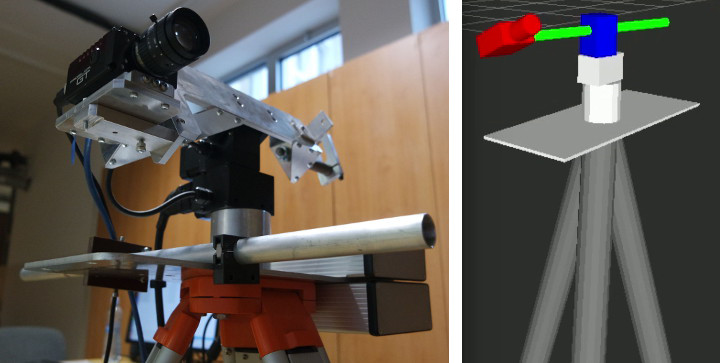
\includegraphics[width=10cm]{fig/camera_unit_photo_model.jpg}
	\caption{A photograph of the upper part of the camera unit consisting of a manipulator Flir PTU-D46-70 with the aluminum mount carrying a camera Prosilica GT 1290C (left) and a corresponding 3D model created for Gazebo simulator (right, see Section \ref{txt:application_of_gazebo}).}
	\label{fig:camera_unit_photo_model}
\end{figure}

\paragraph{manipulator Flir PTU-D46-70} A professional manipulator PTU-D46-70\footnote{A website of product Flir PTU-D46-70: \url{http://www.flir.com/mcs/view/?id=53712}} produced by a well established manufacturer Flir is used (see Figure \ref{fig:prosilica_gt1290c_flir_ptud4670}). As compared to the other professional manipulators this is an entry level device consisting of two stepper motors (pan and tilt axes). The device is capable of maximal angular speed of $60^{\circ}/s$ with the resolution of $0.003^{\circ}$ while the payload must not exceed 4.08 kg \cite{Flir_ptud4670}. The operational range is limited to $[-180^{\circ}, 180^{\circ}]$ in azimuth and $[-47^{\circ}, 80^{\circ}]$ in elevation. The manipulator incorporates no position feedback, the position is inferred from the number of steps and the current resolution, thus it is necessary not to overload the manipulator, otherwise it could loose synchrony and report wrong position. 

\paragraph{camera Prosilica GT 1290C} Prosilica GT 1290C\footnote{A website of product Prosilica GT 1290C: \url{https://www.alliedvision.com/en/products/cameras/detail/1290-1.html}} is an industrial camera manufactured by the Allied Vision company (see Figure \ref{fig:prosilica_gt1290c_flir_ptud4670}). It is a color camera equipped with CCD sensor (type 1/3'') with the resolution of $1280 \times 960$ px and support for $33.3$ FPS and it communicates through gigabit Ethernet \cite{Prosilica_gt1290c}. What is important, the camera natively supports the PTP protocol for precise time synchronization which is a crucial feature in each application relying on stereo vision as it is capable of time synchronization among devices within the range of nanoseconds \cite{PTP}.

%% Photos of Flir and Prosilica.
\begin{figure}[htb]
	\centering
	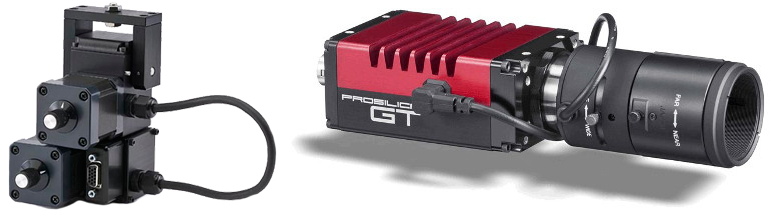
\includegraphics[width=10cm]{fig/prosilica_gt1290c_flir_ptud4670.jpg}
	\caption{Photographs of the manipulator Flir PTU D46-70 (left) and the camera Prosilica GT 1290C (right).}
	\label{fig:prosilica_gt1290c_flir_ptud4670}
\end{figure}

%-------------------------------------------------------------------------
%-------------------------------------------------------------------------
\section{Model} \label{txt:model}

The model of the camera unit is based on the kinematic chain consisting of six joints and five links corresponding to the distance between separate parts of the tripod and separate parts of the manipulator (see Figure \ref{fig:camera_unit_kinematic_chain}). The starting joint \texttt{ground} itself is dependent on the reference location (let us call it \texttt{world}) which represents the origin of the global coordinate frame. The transformation between the \texttt{world} and \texttt{ground} reflects the positioning and heading of the given manipulator within the environment (which is estimated during the stationing process, see Section \ref{txt:stationing_and_rectification}).

The kinematic chain is designed as the composition of transformation matrices where a single joint can be located by applying the Euclidean transformation on the position of the joint it is dependent on. For instance the transformation matrix $M_{cam}$ of the joint \texttt{camera} can be derived as:

\begin{equation}
M_{cam} = M_{ele}T_{cam}R_{Z_{cam}}R_{X_{cam}}R_{Y_{cam}},
\end{equation}

where $M_{ele}$ is the transformation matrix of the joint \texttt{ele} which the joint \texttt{camera} is dependent on, and $T_{cam}$ and $R_{AXIS_{cam}}$ are transformation and rotation matrices describing transformation from the joint \texttt{ele} to the joint \texttt{camera}. 

%% A schema of the camera unit - kinematic chain.
\begin{figure}[htb]
	\centering
	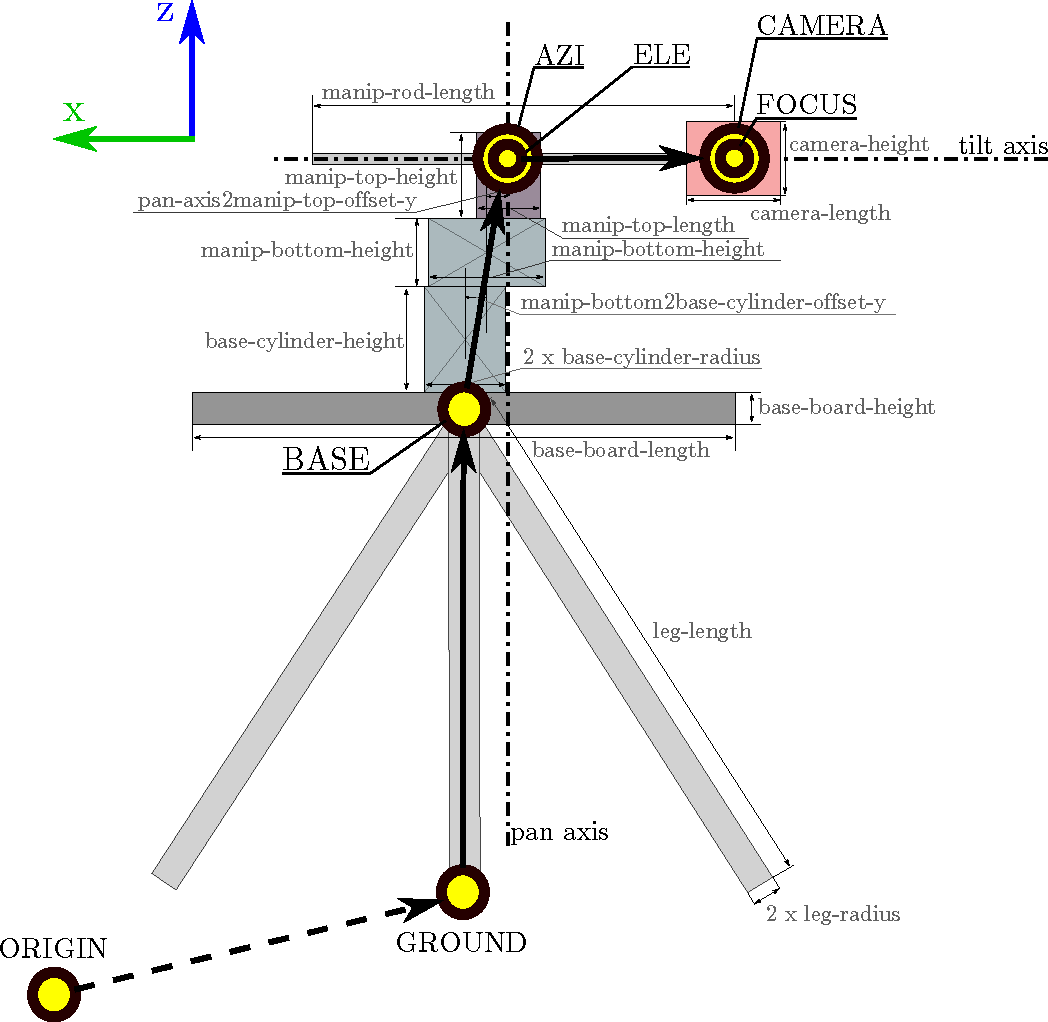
\includegraphics[width=14cm]{fig/camera_unit_kinematic_chain.pdf}
	\caption{Schematic view of the kinematic chain of a camera unit with the joints depicted by the yellow circles with black crosses. The sizes of all components necessary to specify the translation matrices between consecutive joints are shown as well. Note that this is the rear view, i.e. the camera is seen from behind. Thus the joints \texttt{camera} and \texttt{focus} overlap as they both lie on the optical axis (the joint \texttt{focus} has a lower value of the Z coordinate).}
	\label{fig:camera_unit_kinematic_chain}
\end{figure}


%=========================================================================
%=========================================================================
\chapter{Stationing, Rectification and Calibration} \label{txt:stationing_and_rectification}
% 2,5 - 3,5 ns

The precision of the whole system is dependent on the uncertainty of the system input as well as on the imprecision of the camera unit construction. The process of stationing aims to alleviate the uncertainty of the system input while the main purpose of the rectification is to reduce the difference between the real camera unit and its model.

%-------------------------------------------------------------------------
%-------------------------------------------------------------------------
\section{Stationing}

Since the stationing is considered to be already a working subsystem of the whole project (and thus is not dealt with within the scope of this work) only the main principle will be briefly described. The stationing is composed of two parts: finding the geographical north and finding the relative azimuthal and elevation angles between each pair of camera units.

%.........................................................................
%.........................................................................
\subsection{Geographical North} \label{txt:geographical_north}

Though it is a common practice to estimate the heading\footnote{Heading is the term used to describe the angle between the torso of the human body and the geographical north \cite{Henriksson648760}} using a magnetometer, this device is unsuitable for this project since the accuracy of the current professional class magnetometers is insufficient. For instance the accuracy of the magnetometers meant for compassing applications produced by Honeywell company range from hundreds to thousands of milliradians \cite{Honeywell:compassing_catalog}.

In order to find the orientation of each camera unit placed in the outdoor environment, distinctive landmarks (created either by human or nature) with known geographical positions are used. For each such landmark, the manipulator is rotated so that the optical axis of the camera would intersect that landmark and both the azimuth and elevation value is registered. Using triangulation the geographical position of the camera unit is derived. 

A different possible approach takes advantage of the celestial objects, such as the moon, sun or stars for which the current geographical position is known as well. Nevertheless, this approach can only be used between the sunset and the dawn.

%.........................................................................
%.........................................................................
\subsection{Relative Azimuth and Elevation}

To further reduce the impact of the uncertainty of the system input produced by the GPS and the system error given by the imprecision of the heading estimation (see Section \ref{txt:geographical_north}) it is convenient to find the relative position of each camera unit with regards to the rest of the camera units.

The information about the geographical position of all camera units as obtained from the GPS sensors is distributed across the whole system. Each pair of camera units then automatically performs the following:

\begin{enumerate}
	\item Set the azimuth and elevation of the manipulator so that the optical axis of the camera would intersect the expected location of the LED target of the other camera unit.
	\item Using the visual clue adjust the azimuth and elevation so that the optical axis of the camera would intersect the center of the LED target of the other unit (see Figure~\ref{fig:stationing_aiming}).
	\item Save the current azimuth and elevation values of both camera units and use those values to update the model of the system.
\end{enumerate}

%% Stationing process of one pair of the camera units
\begin{figure}[htb]
	\centering
	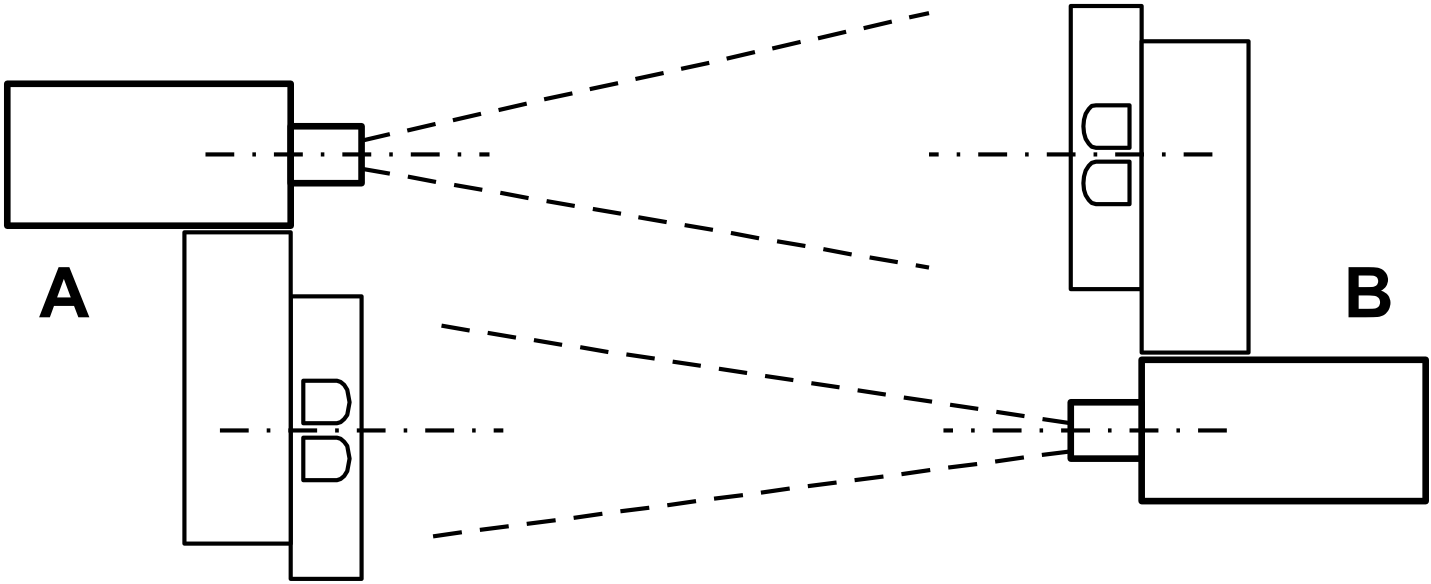
\includegraphics[width=8cm]{fig/stationing_aiming.png}
	\caption{Schema of the stationing process where two camera units attempt to align the optical axes of their cameras so that they would intersect the LED target of the other unit.}
	\label{fig:stationing_aiming}
\end{figure}


%.........................................................................
%.........................................................................
\subsection{Horizontality}
Since the camera unit is expected to be placed in an unknown outdoor terrain, it will never stand on an ideally horizontal surface. Therefore, it is necessary to either ensure that the unevenness of the surface is compensated by the suitable setting of the camera unit's stand or both the side tilt and front tilt angles of the stand must be estimated and integrated to the model of the given camera unit. For these purposes the inclinometer attached to the base plane of the camera unit (see Section \ref{txt:camera_unit}) is used.


%-------------------------------------------------------------------------
%-------------------------------------------------------------------------
\section{Rectification}

The process of rectification serves the purpose of reducing the system error caused by the imprecise attachment of the camera to the manipulator. The model of the camera unit assumes that the camera is precisely attached to the manipulator so that the camera image sensor is positioned perpendicular to the azimuthal axis and the rows of the image sensor are parallel to the elevation axis (i.e. the camera is not rotated along the optical axis).

Regarding these requirements the rectification consists of three parts: rotation along the optical axis, rotation along the azimuthal axis, finding the default elevation angle.


%.........................................................................
%.........................................................................
\subsection{Rotation Along the Optical Axis}

A custom made metal mount is attached to the bottom side of the camera. The mount is then attached to the manipulator using two opposing round tenons enabling for the rotation of the mount (together with camera) along the axis parallel to the optical axis of the camera (see Figure \ref{fig:rect_model_front_view}).

%% The front view of the model of the camera unit
\begin{figure}[htb]
	\centering
	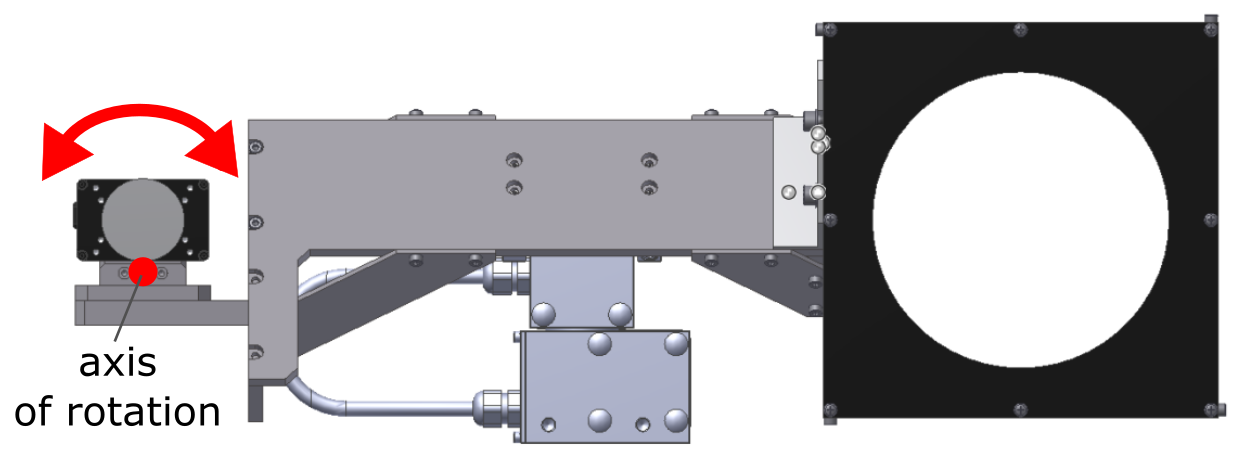
\includegraphics[width=10cm]{fig/rect_model_front_view.png}
	\caption{Front view of the top part of the camera unit. The red arrow shows the possible rotation of the camera along the axis parallel to the optical axis. The Figure is adopted from company Oprox, a.s.}
	\label{fig:rect_model_front_view}
\end{figure}

In this part the rectification target with three parallel horizontal black lines is used. Each line has a different width so that the operator can select the most suitable one (given the distance of the target, ambient lighting conditions, etc.). As the first step a surveying automatic level is used to rotate the target so that the black lines become horizontal. Then the camera is pointed approximately to the center of the target. The camera image stream is blended with the same stream mirrored across the vertical axis. The operator then manually rotates the camera so that the black lines in this blended image stream appear visually aligned (see Figure \ref{fig:rect_mirrored_stream}). Once set, the mount with the camera is fixed to the manipulator using two set screws.

%% Rectification of the rows of the camera image sensor - original stream blended with the mirrored stream
\begin{figure}[htb]
	\centering
	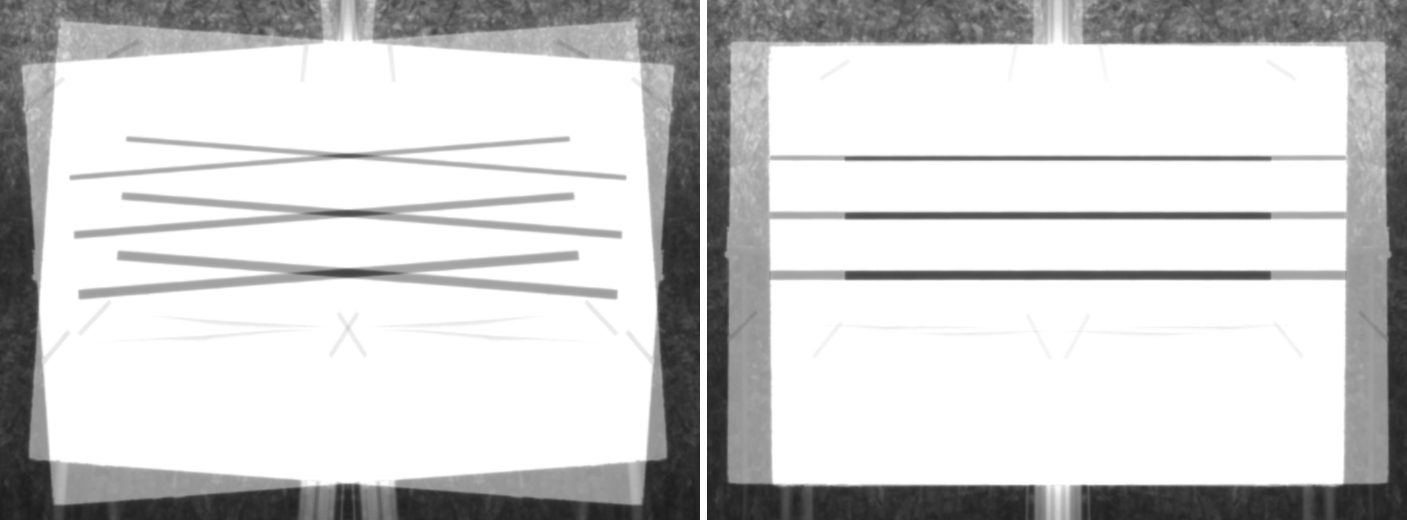
\includegraphics[width=12cm]{fig/rect_mirrored_stream.png}
	\caption{A blended image stream from the camera before (left) and after (right) rotating the camera along the optical axis to the correct position.}
	\label{fig:rect_mirrored_stream}
\end{figure}

%.........................................................................
%.........................................................................
\subsection{Rotation Along the Azimuthal Axis}

The mount can still rotate along the axis parallel to the azimuthal axis (see Figure \ref{fig:rect_model_top_view}). It is necessary to ensure that the optical axis of the camera is perpendicular to the elevation axis. 

%% The top view of the model of the camera unit
\begin{figure}[htb]
	\centering
	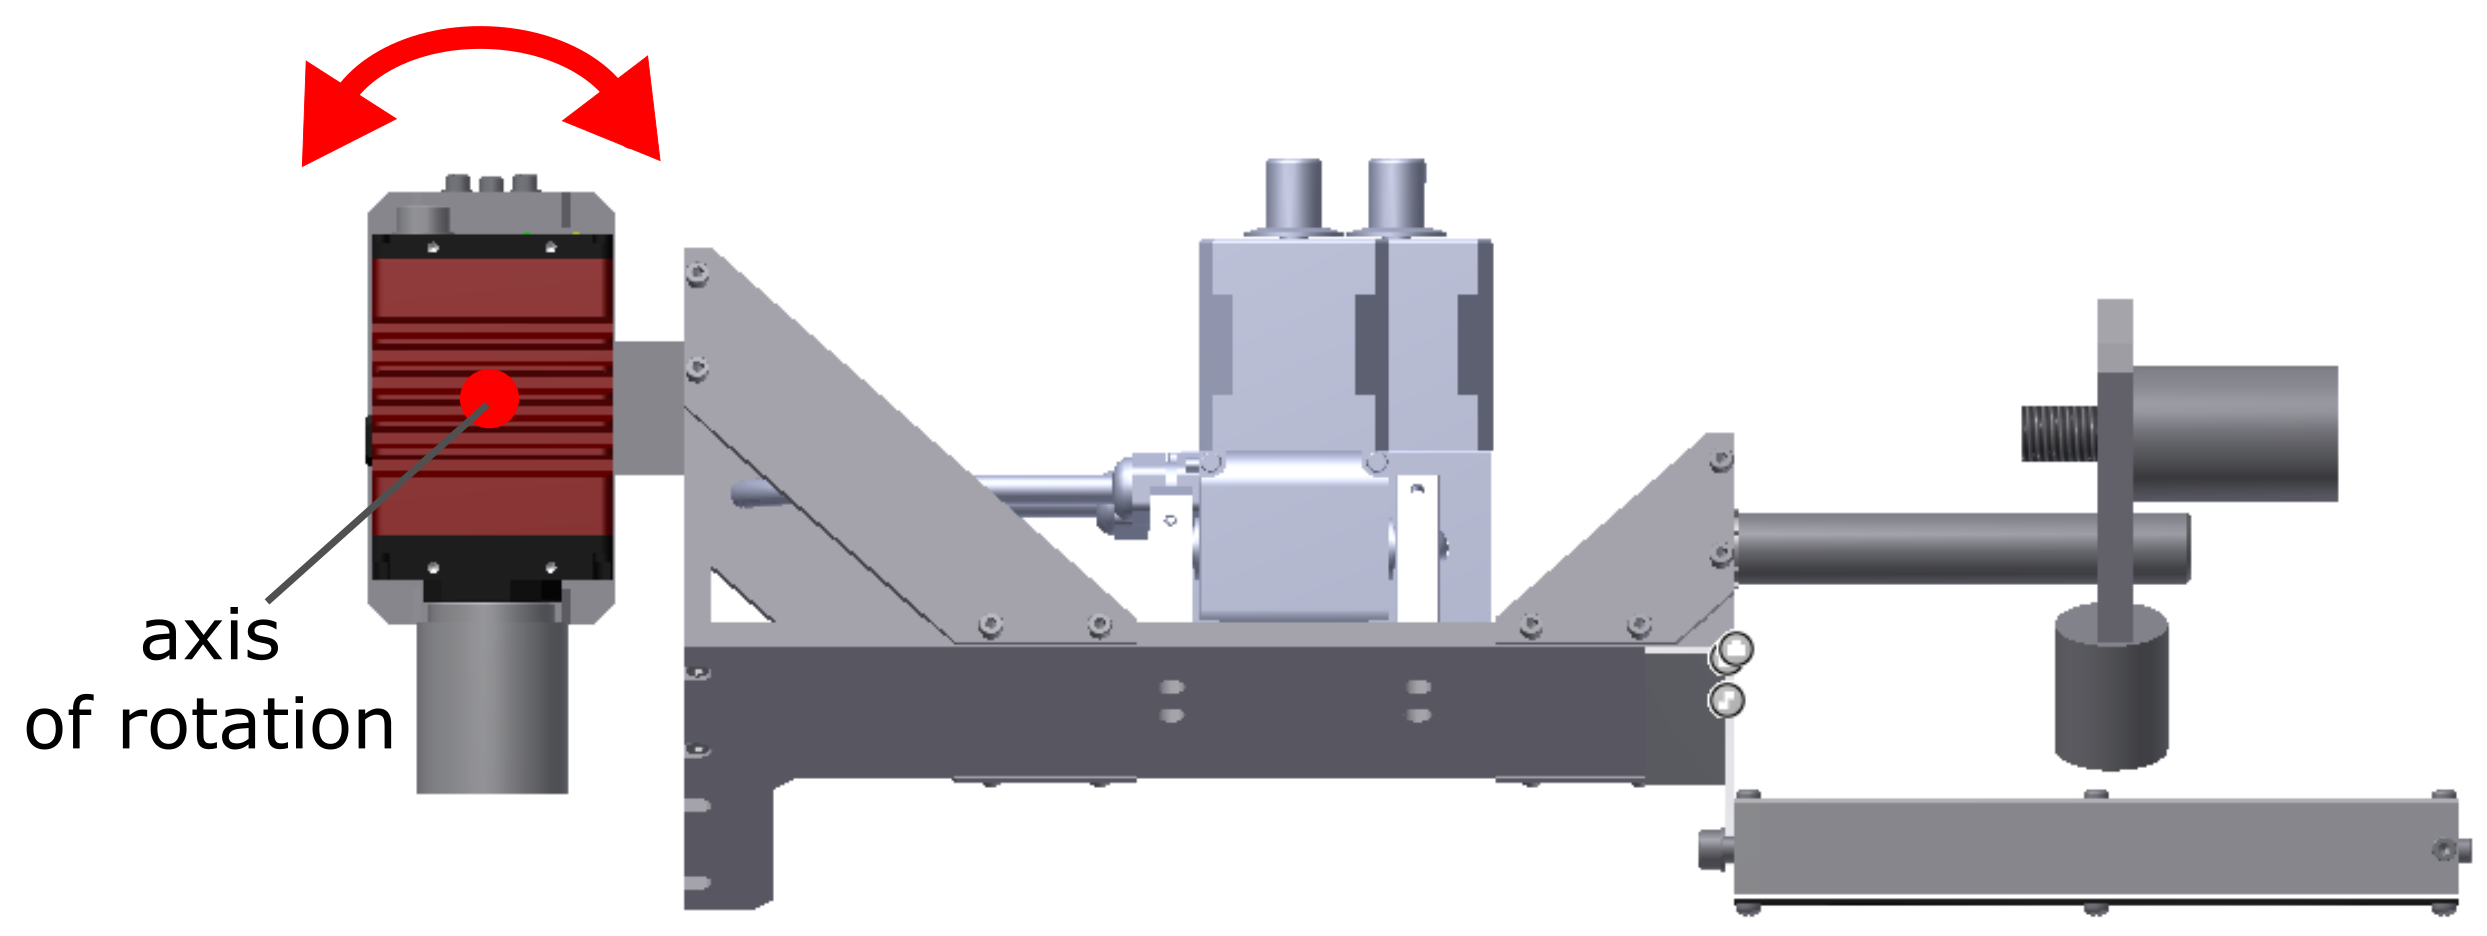
\includegraphics[width=11cm]{fig/rect_model_top_view.png}
	\caption{Top view of the top part of the camera unit. The red arrow shows the possible rotation of the camera along the axis parallel to the azimuthal axis. The Figure is adopted from company Oprox, a.s.}
	\label{fig:rect_model_top_view}
\end{figure}

The same target from the first part of the rectification is used, but two black crosses are added to the selected horizontal black line. The distance $d_{ao}\ m$ between two crosses equals to the distance between the azimuthal and optical axis (which is known from the engineering design, see Figure \ref{fig:rect_azi_axis}). 

%% Photograph of the camera unit with the telescope mounted on the top
%% Screenshot of the digital crosshair and the offset
\begin{figure}[htb]
	\centering
	\begin{minipage}{.37\textwidth}
		\centering
		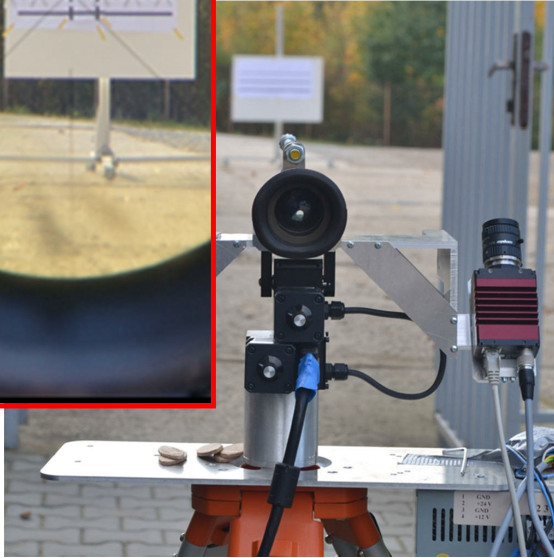
\includegraphics[width=.99\linewidth]{fig/rect_telescope.png}
		\captionof{figure}{A telescope mounted on top of the manipulator. A person looking through a telescope sees a crosshair.}
		\label{fig:rect_telescope}
	\end{minipage}
	\hfill
	\begin{minipage}{.59\textwidth}
		\centering
		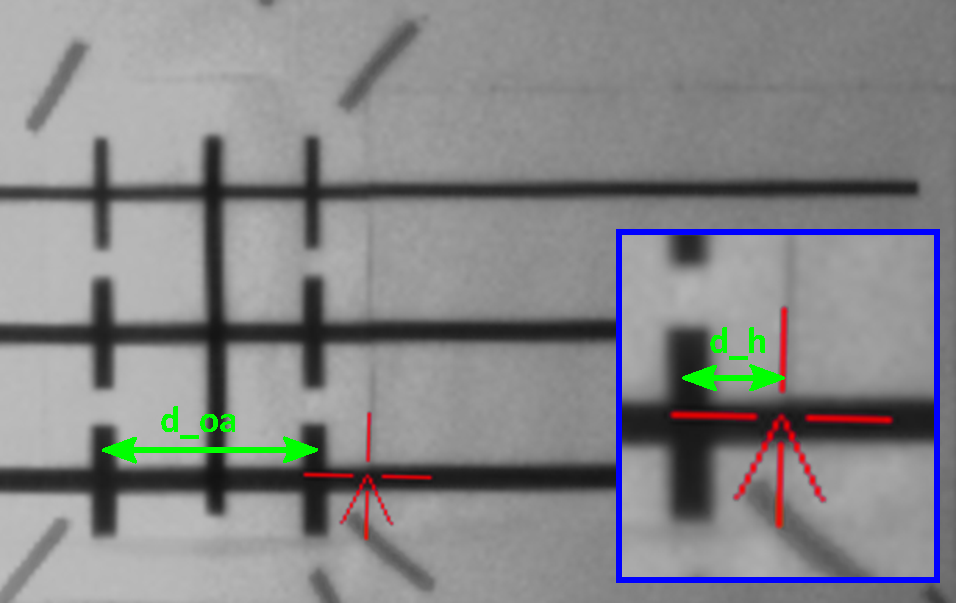
\includegraphics[width=.99\linewidth]{fig/rect_azi_axis.pdf}
		\captionof{figure}{Rectification target with the pairs of black crosses. The two crosses in a pair are $d_{ao}\ m$ appart. A digital corsshair is displayed in order to find the horizontal offset $d_{h}$.}
		\label{fig:rect_azi_axis}
	\end{minipage}
\end{figure}

A military optical monocular telescope (see Figure \ref{fig:rect_telescope}) is mounted on top of the manipulator. The optical axis of the telescope intersects the azimuthal axis, it is perpendicular to it and it intersects the left cross of a given pair on the rectification target. The camera is rotated so that its optical axis (represented by the digital crosshair) intersects the right cross on the target and then it is fixed using set screws. As the screws are tightened the camera is unintentionally rotated a bit again which causes the visual offset between the crosshair and the cross on the target. The offset expressed in pixels is recorded and transformed to the default angle $\beta$ expressed in milliradians (see Figure \ref{fig:rect_pixel_offset}) of rotation along Z-axis of the joint \texttt{camera} in the camera unit model (see Section \ref{txt:camera_unit}):

\begin{equation*}
\begin{aligned}
\beta &= \arccos\frac{focal\_length}{offset}, \\
offset &= pixel\_offset * pixel\_size
\end{aligned}
\end{equation*}

%% Geometry schema showing how to calculate angle beta - pixel offset
\begin{figure}[htb]
	\centering
	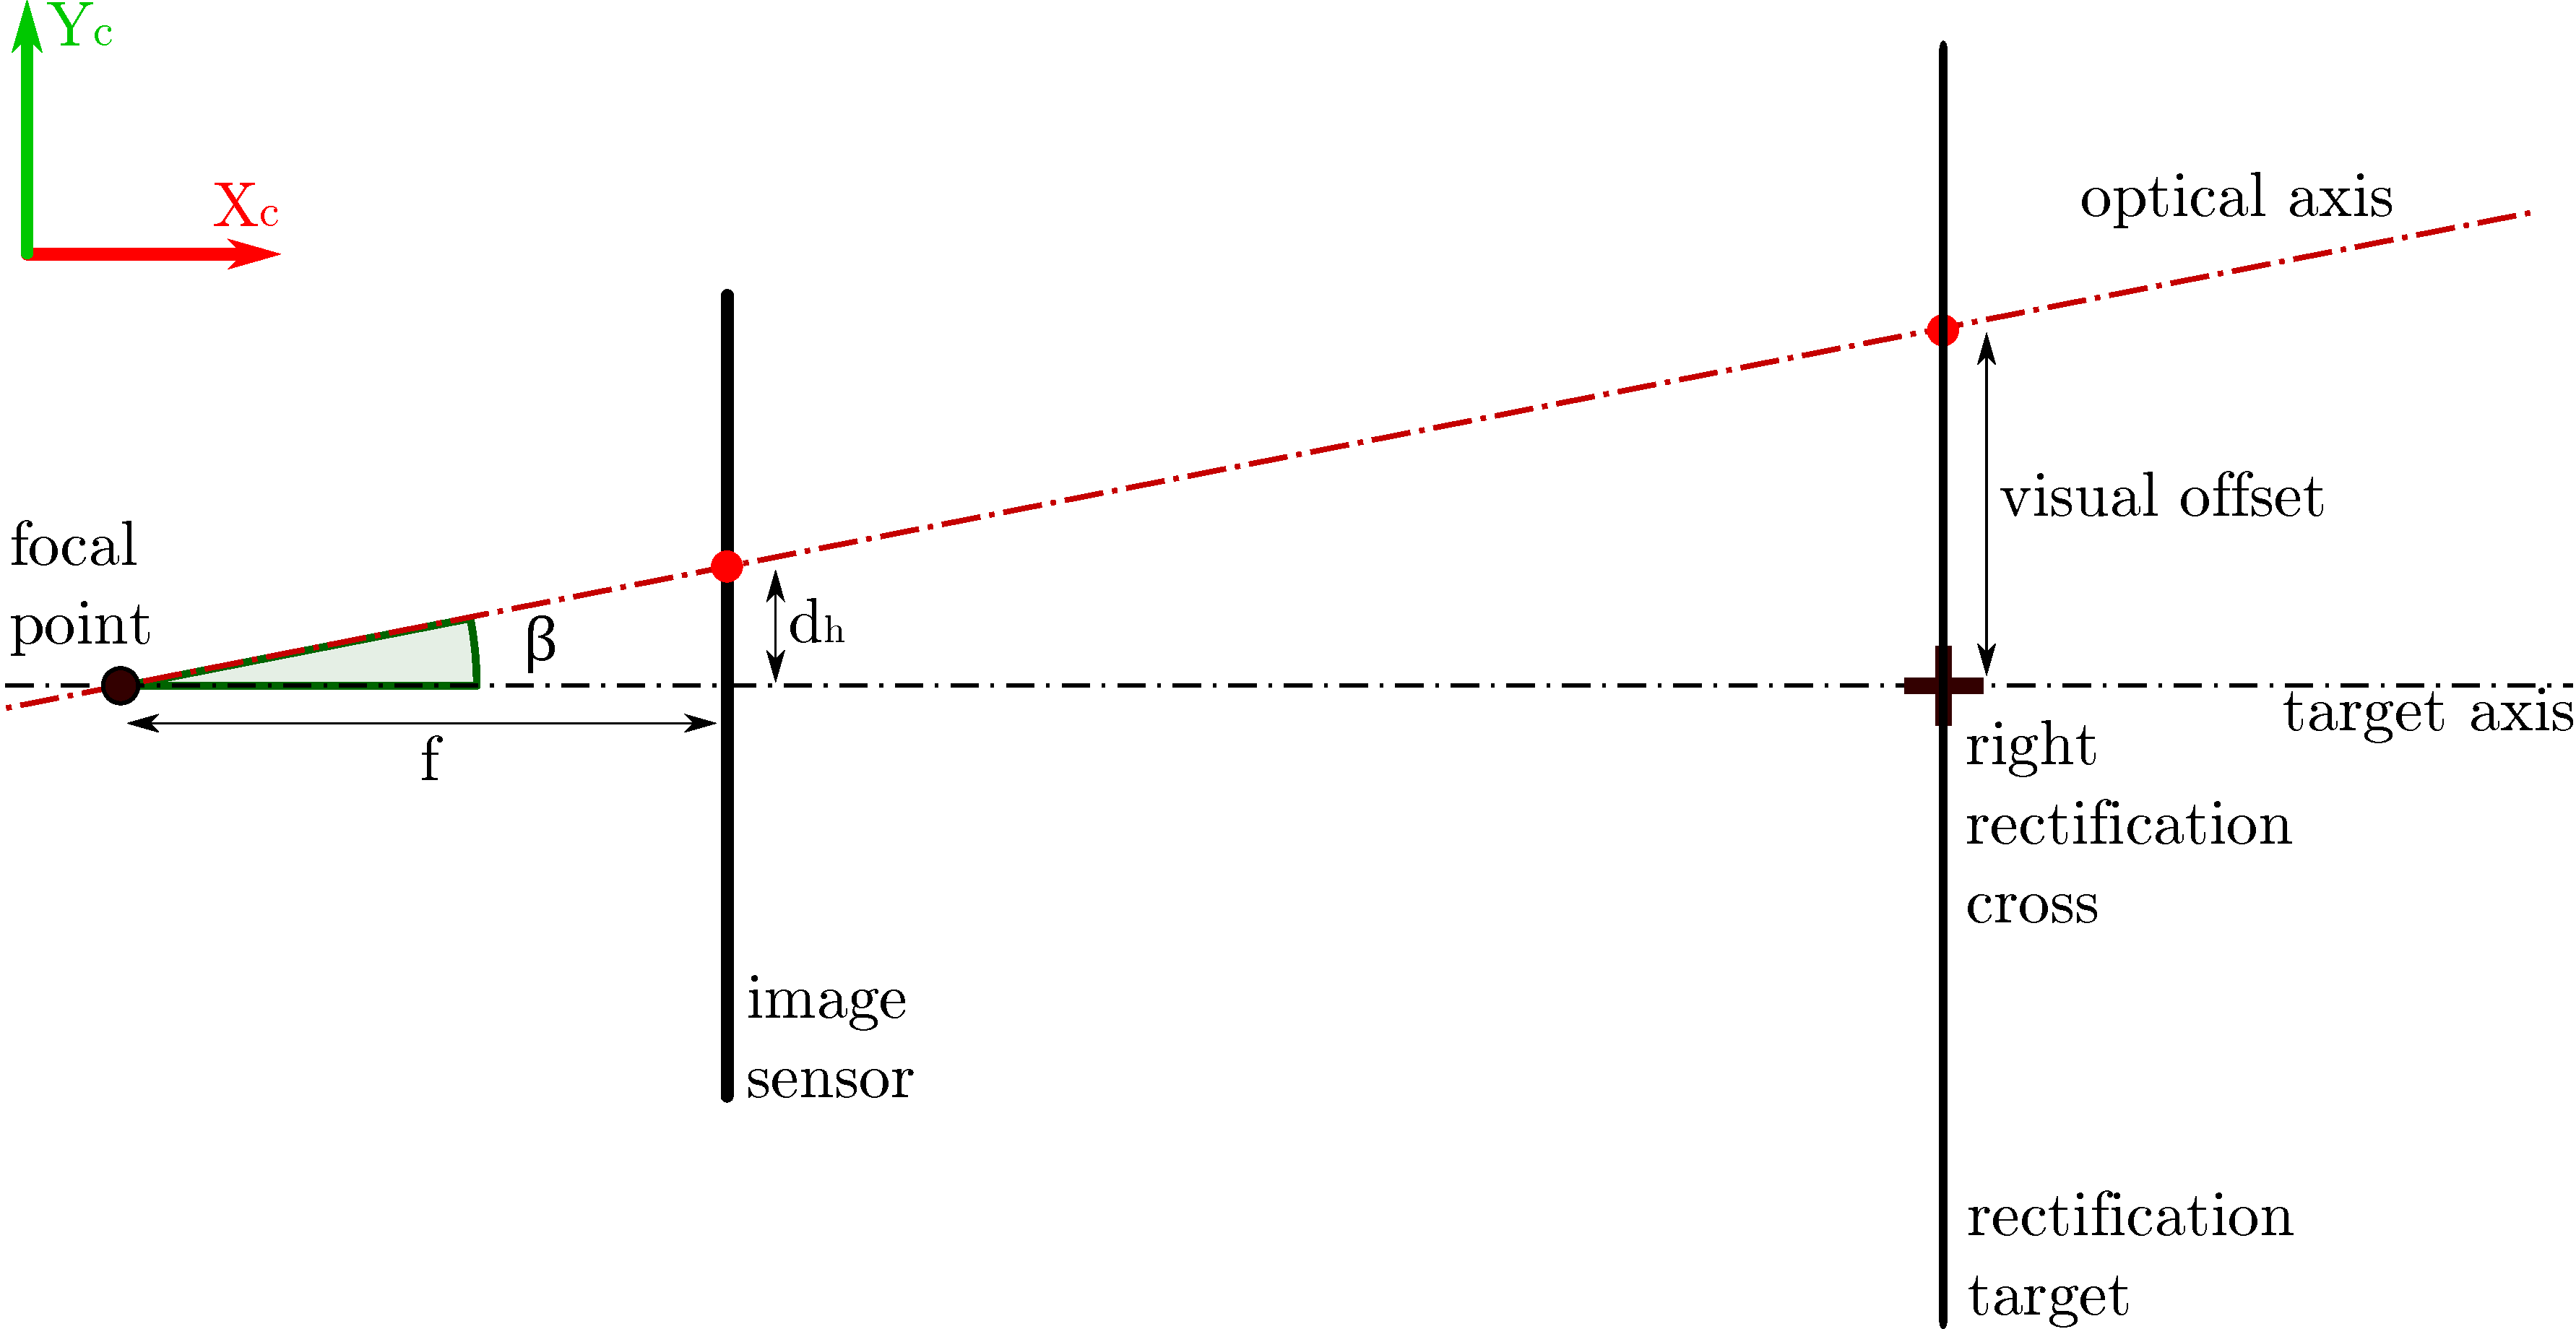
\includegraphics[width=13cm]{fig/rect_pixel_offset.pdf}
	\caption{The top view schema of a rectification target being projected to the image sensor of the camera. The value of the angle $\beta$ is one of the output of the rectification process.}
	\label{fig:rect_pixel_offset}
\end{figure}


%.........................................................................
%.........................................................................
\subsection{Finding the Default Elevation Angle}

Given the application of the system the camera is expected to mainly observe the sky. Considering the limited elevation range of the manipulator \texttt{Flir PTU D46-70} (see Section \ref{txt:camera_unit}), the camera must be mounted to the manipulator with the default elevation angle approximately $-60^{\circ}$. However, after fixing the camera it is necessary to find default elevation angle precisely. 

For this purpose a pair of rectification targets, which consist of vertical black and white lines representing the marks of a ruler. The targets are positioned in a row with the distance of a few meters so that the front target would overlap approximately half of the rare target when observed from the camera. Both targets must be rotated so that the lines become horizontal, then the operator manually adjusts the elevation of the manipulator so that the digital crosshair would intersect the same mark on both targets where the two marks form a straight line (see figure \ref{fig:rect_default_elevation_angle}). Once found the current elevation angle is recorded and integrated to the model of the camera unit as an angle of rotation along the Y-axis of the joint \texttt{camera} (see Section \ref{txt:camera_unit}).

%% The rectification target for finding the default elevation angle.
\begin{figure}[htb]
	\centering
	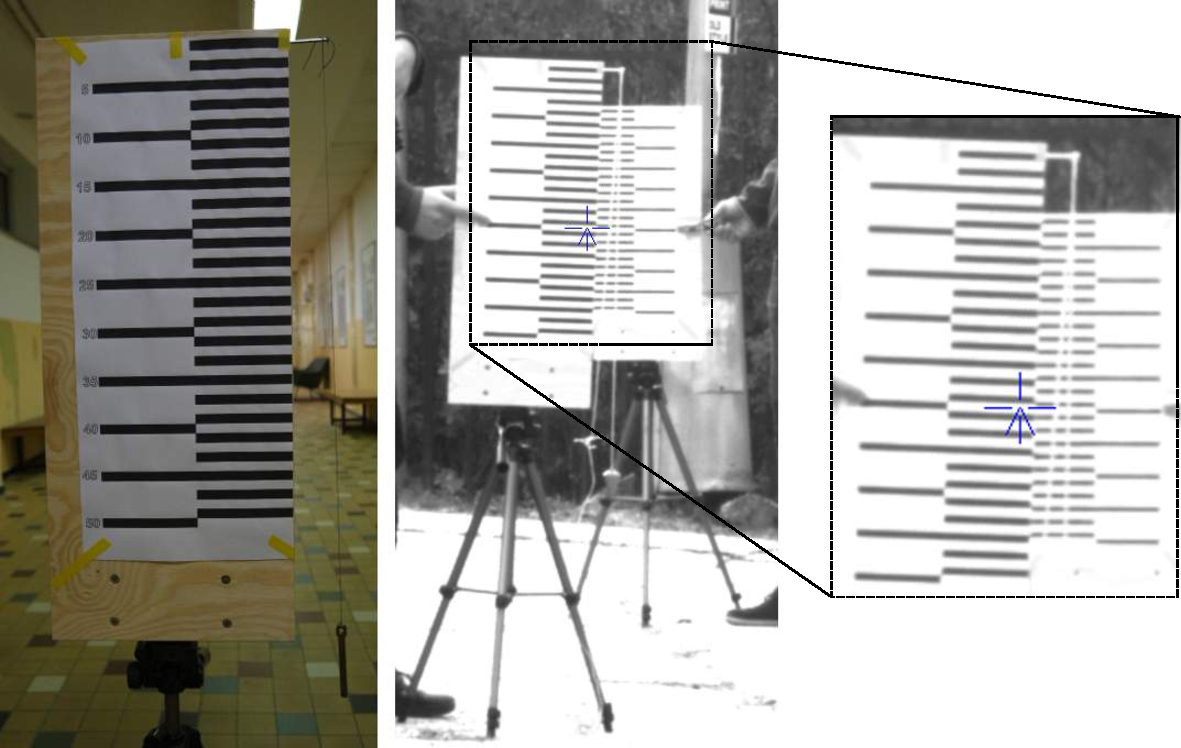
\includegraphics[width=13cm]{fig/rect_default_elevation_angle.pdf}
	\caption{Front target of a pair of the rectification targets used to find a default elevation angle (left). A screenshot from the image stream of the camera with the crosshair focused on a row where the marks of the rulers align (right).}
	\label{fig:rect_default_elevation_angle}
\end{figure}

%-------------------------------------------------------------------------
%-------------------------------------------------------------------------
\section{Calibration}

%=========================================================================
%=========================================================================
\chapter{Object Tracking in Multi-camera System}

This section discusses the various approaches for detection and tracking of the objects using the computer vision techniques. First the importance of the suitable object representation is explained, then the detection and tracking algorithms are described.

%-------------------------------------------------------------------------
%-------------------------------------------------------------------------
\section{Object Model}

Choosing a suitable representation of an object of interest is a first step when designing a tracker. It is a crucial task since the choice of the features determines the type of the final tracker due to the strong relationship between the algorithm and the representation of the object and it can significantly impact the overall performance of the tracker. There are two main representations, the \textit{shape} and the \textit{appearance} \cite{Yilmaz:2006:OTS:1177352.1177355}.

\paragraph{shape representation} 
This category covers the use of points, geometric shapes, silhouettes and contours, articulated models and skeletal models. The point representation is not suitable for OLS since the distant aerial objects appear relatively small in the image and might not provide enough distinctive points. The geometric shapes seem suitable as long as the aerial object is far enough so that it could be approximated by a primitive geometric shape. Silhouettes and contours are mostly used for tracking non rigid objects (which is not the case of OLS), neither articulated model is needed to describe an UAV. Considering the small size of the object of interest, a skeletal model would most probably degrade to a single line or a point.

\paragraph{appearance representation} 
The second category covers the use of templates, active appearance models and multiview appearance models. Active appearance models seem promising since they simultaneously model the object shape and appearance, however there is a need for an offline training phase. The templates combine the spatial and appearance information and can scale well to support varying object size (UAV approaching or flying away). A multiview appearance model might perform even better since it is designed to be robust against variation of the appearance of one object due to the change of its orientation.

%%-------------------------------------------------------------------------
%%-------------------------------------------------------------------------
%\section{Detection}
%
%Before a tracking of the object can be initiated, the object of interest must first be discovered, which is the main task of object detectors. Even though the OLS allows a human operator to interfere and manually select an object for tracking, the system should be able to perform fully autonomously as well. The approaches to detect an object can be divided into two categories based on the appearance of the object, where the first group covers the cases where the system already posses a strong information about the objects since they incorporate artificial landmarks, while the second group relies merely on the natural appearance and has only limited or no prior knowledge about the objects \cite{Multi-Camera_Sensor_System_for_3D_Segmentation}. Since the OLS aims on tracking unknown UAVs the first group of approaches is out of question.
%
%A couple of approaches can be distinguished among the detectors using natural appearance \cite{Yilmaz:2006:OTS:1177352.1177355}:
%
%\paragraph{detection of points} This approach goes with the shape representation of the object given by the keypoints. Among others the Harris corner detector or SIFT and SURF descriptors are widely used.
%
%\paragraph{background modeling} Under the assumption an observed scene does not change rapidly its appearance can be learned resulting in a background model. The task of the object detector is then to estimate for each subregion or even each pixel whether it belongs to a background or to a foreground (i.e. the object of interest). A widely used approach is to model each pixel as a mixture of Gaussians (in order to support a periodically changing background). Another possible solution is to model intensity variations of separate pixels as the states (including both \textit{background} and \textit{foreground} state) and then with the help of Hidden Markov Models to estimate the state a given pixel is currently in. Since it is possible to enhance these algorithms to allow for the camera motion (resulting in the change of the camera view) they seem suitable for the OLS system. 
%
%\paragraph{supervised classification} If the (coarse) class of the objects to be tracked is known beforehand and a proper dataset is available, a classifier can be trained to detect the objects. Among others, the neural networks or adaptive boosting methods are widely used. Since the OLS aims to localize UAVs, the utilization of a classifier seems like a suitable solution.

%-------------------------------------------------------------------------
%-------------------------------------------------------------------------
\section{Visual Tracking}

The main purpose of the tracker is to iteratively estimate the trajectory of the tracked object from frame to frame and regarding the approaches the trackers can be divided into three main categories \cite{Yilmaz:2006:OTS:1177352.1177355}:

\paragraph{point tracking} 
The tracker detects the keypoints in each frame, selects those representing the object and computes the transformation from the previous frame.

\paragraph{kernel tracking} 
This approach corresponds to a representation of an object using a template, where kernel is the description of both shape and appearance.

\paragraph{silhouette tracking}
Silhouettes representing the object can be tracked either by shape matching or contour evolution. \\

Since the representation by a template (or multiple templates) suits conditions of the OLS the best, an approach Tracking Learning Detection belonging to the \textit{kernel tracking} category was chosen to perform the tracking of the object of interest. TLD is one of the best performing state-of-the-art algorithms developed for tracking general objects and its capabilities seem promising for the needs of OLS. For detailed description of the algorithm see Section \ref{txt:tracking_learning_detection}.

%.........................................................................
%.........................................................................
\subsection{Tracking-Learning-Detection} \label{txt:tracking_learning_detection}

The Tracking Learning Detection (TLD) \cite{Kalal:2012:TRA:2225045.2225082} is an algorithm designed for performing so called long-term tracking, a robust tracking of an object which might change its appearance, be temporarily occluded by closer objects or temporarily completely disappear from the scene. Since this task cannot be achieved solely neither by a tracker nor by a detector, the TLD aims to combine the strengths of the detection and tracking algorithms by combining their results. Furthermore the algorithm incorporates the online adaptation subsystem capable of learning the new appearances of the tracked object in the course of the tracking.

A conceptual diagram of the TLD algorithm is shown in Figure \ref{fig:tld_block_diagram}. The \texttt{tracking} component tracks the object and for each frame produces the new position. It expects that object does not disappear (occlusion, out of FOV) from the scene and if it does, the tracker fails. The \texttt{detection} component performs full scanning of the image for each frame. It detects the object and if needed it reinitializes the tracker. The \texttt{learning} component is capable of generating new appearances of the tracked object and thus improving the performance of the detector. 

The object itself is modeled as a set of patches, each patch being already learned appearance represented by the rectangular bounding box around the object rescaled to a normalized resolution of 15 x 15 pixels. The similarity of the patches is given by the normalized cross-correlation.

%% TLD block diagram
%% TLD PN learning block diagram
\begin{figure}[htb]
	\centering
	\begin{minipage}{.34\textwidth}
		\centering
		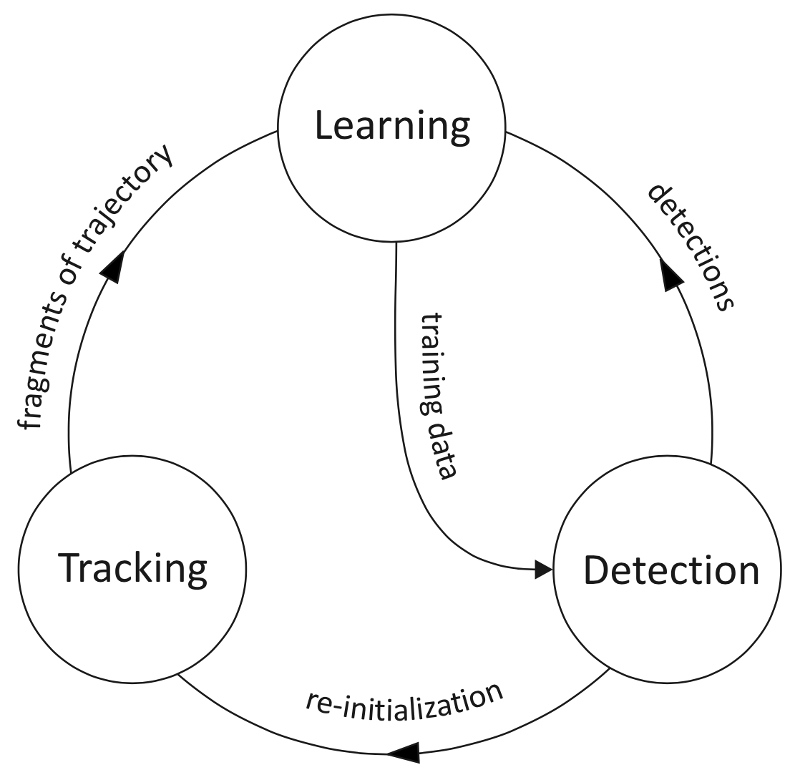
\includegraphics[width=.99\linewidth]{fig/tld_block_diagram.png}
		\captionof{figure}{A diagram of the main TLD components. Image is adopted from \cite{Kalal:2012:TRA:2225045.2225082}.}
		\label{fig:tld_block_diagram}
	\end{minipage}
	\hfill
	\begin{minipage}{.63\textwidth}
		\centering
		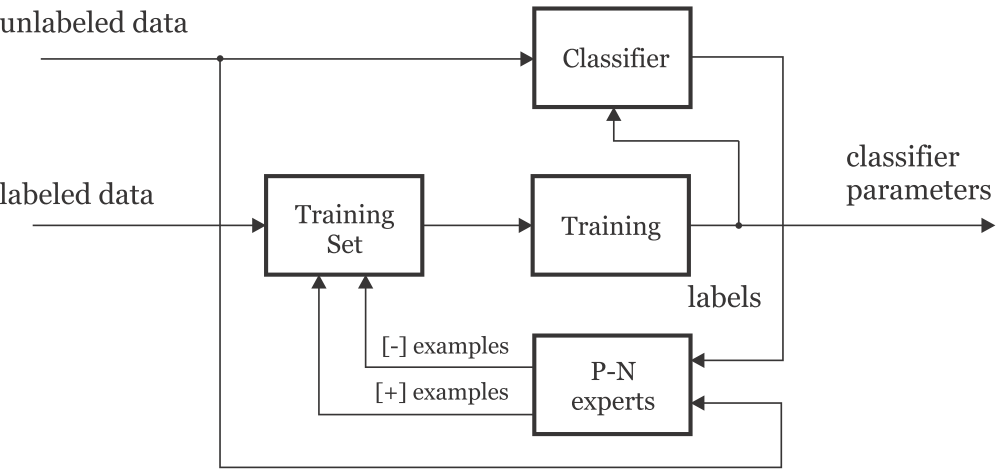
\includegraphics[width=.99\linewidth]{fig/tld_pn_learning_block_diagram.png}
		\captionof{figure}{A diagram of the PN learning process. Image is adopted from \cite{Kalal:2012:TRA:2225045.2225082}.}
		\label{fig:tld_pn_learning_block_diagram}
	\end{minipage}
\end{figure}

\paragraph{Detection} Detector treats each frame as an independent one and scans a full image. A scanning window is used and it is gradually scaled (in order for the detector to achieve scale invariance) and iteratively shifted along a regular grid of candidate positions. Since this task is computationally intensive a cascade classifier is used so that the detector could quickly decide whether a given subregion contains the object. In case of TLD, the cascade classifier consists of three sequential stages specifically ordered so that earlier the stage is the more subregions it should reduce while being computationally less expensive. Should the subregion be rejected by any stage, later stages ignore it completely.

\paragraph{Tracking} The tracking subsystem is based on the algorithm called the Median-Flow tracker. A $10 \times 10$ grid is used to select the positions within the bounding box representing the object. For each position a given point is tracked between the consecutive frames using pyramidal Lucas-Kanade tracker and eventually the tracker only accepts a 50\% of the most reliable displacements to estimate a new position of the target.

\paragraph{Learning} Since the classifier used in the detection phase is initially trained using only one positive patch (the initial bounding box selected by a user) it tends to make errors as a video stream progress since the moving object of interest change its appearance due to the transformation caused by its motion. Therefore an online so called \texttt{P-N learning} component is incorporated in the system which gradually extends the training sets. Two experts are used, a \texttt{P-expert} identifies only false negatives while \texttt{N-expert} identifies only false positives. Once a wrongly classified patch is found, the experts extend the training set and the classifier is retrained (see Figure \ref{fig:tld_pn_learning_block_diagram}).

%.........................................................................
%.........................................................................
\subsection{Tracking Using Background Modeling and Particle Filter}
 
\vata[18]
 
%=========================================================================
%=========================================================================
\chapter{Occlusion Detection Using 3D Environment Reconstruction}

\vata[23]

%=========================================================================
%=========================================================================
\chapter{Target Localization Using Triangulation}

\todo{LOKALIZACE OBJEKTU VE VICEKAMEROVYCH SYSTEMECH}
\todo{ALGORITMY VHODNE PRO RESENI ULOHY}

- Cameras are modeled as pinhole cameras. This is a simple model that describes the mathematical
relationship between the coordinates of a 3D point in the camera coordinate system and its
projection onto the image plane in an ideal camera without lenses through the expressions in 

\todo{== (obrazek z rvizu (protnuti primek) ==}

 Given  the  extrinsic  and  intrinsic  camera 
 parameters,  each  image  point  defines  a  ray  in  three 
 dimensional spaces, and in the absence of measurement errors, 
 all  rays  from  different  cameras  intersect  in  the  same  object 
 point. But actually the four rays may not intersect in the same 
 point  due  to  the  low-quality  video  cameras  and  other 
 complicated  reasons.
 
 \vata[28]

%=========================================================================
%=========================================================================
\chapter{Implementation} \label{txt:implementation}
% 2 - 4 ns

The whole system is built on the robotic framework Robot Operating System (for details see Section \ref{txt:robot_operating_system}). Since the ROS defines multiple conventions, restrictions and best practices the whole system design including the selection of a programing language, a programing and a communication paradigm, a target platform and a tool for physical simulations is impacted by the possibilities of this framework.

As of writing this text a current state of the implementation mainly builds on the virtual environment provided by the physical simulator Gazebo (see Section \ref{txt:application_of_gazebo}). When confronted with the overview of all subsystems making up the whole system presented in Section \ref{txt:system_overview}, so far the following parts are already designed, implemented and/or integrated:

\begin{itemize}
\item manual control of the manipulator using peripheral devices
\item manual selection of a target and distribution of its appearance to all CUs
\item integration and utilization of a OpenTLD tracker
\item the first prototype of triangulation of a 3D positions of a target within global frame
\item integration of all subsystems
\end{itemize}

Furthermore a few additional tools were utilized and/or implemented as the necessary building blocks allowing for further development and testing:

\begin{itemize}
\item a functional model of a whole system in Gazebo environment
\item a standalone application for rectification
\end{itemize}


%-------------------------------------------------------------------------
%-------------------------------------------------------------------------
\section{Robot Operating System} \label{txt:robot_operating_system}

Despite its name the ROS\footnote{The official website of ROS: \url{http://www.ros.org}} is not an operating system but rather a collection of open source libraries, tools and conventions which serve the purpose of a middlewear running alongside a real operating system, however it provides the programmer with the hardware abstraction,  low-level device control, implementation of commonly-used functionality,
message-passing between processes, and package management \cite{O'Kane201310}.

Since the original motivation for developing ROS was to support the collaboration among the experts in the field of robotics in the means of a common software platform~\cite{ROS-an-open-source-Robot-Operating-System}, a huge developer community has formed around ROS which resulted in wide-scale penetration of this framework as well as the support for a huge range of hardware devices.

%.........................................................................
%.........................................................................
\subsection{Application of ROS}

The OLS is designed to become a relatively complex system, thus it exhibits non-trivial implementation requirements such as a need to distribute the computation among multiple computers, the real time performance, integration with physical simulator, etc. Since ROS is a mature framework satisfying the most of theses requirements (see Table \ref{tab:ols_requirements_ros_features}), it was chosen as a main implementation platform.


{\renewcommand{\arraystretch}{1.5}
\begin{table}[htbp]
	\centering
	\caption{The table lists the most important requirements of the OLS and describes how the ROS framework addresses them.}
	\begin{tabularx}{0.99\textwidth}{XX}
		\toprule
		\textbf{OLS requirements} & \textbf{ROS features} \\
		\midrule
		native support for hardware such as Prosilica camera, manipulator Flir PTU D46-70, joystick, keyboard & nodes implementing image capture from Prosilica cameras, capturing events from keyboards and joysticks \\
		modularity and reusability of source code & each subsystem is represented by a separate process (node), straightforward reusability \\
		distribution of computation among multiple computers & provides abstraction layer for distributing nodes across devices \\
		simple data exchange among subsystems & the publisher/subscriber paradigm \cite{O'Kane201310}, support for custom message formats \\
		real time performance & C++ implementation \\
		modelling and simulating the robot & custom language \texttt{URDF}\footnotemark ~for robot modeling, integration with Gazebo \\
		specifying a kinematic chain, heavy 3D transformation computation & native support for computing transformation between frames using package \texttt{tf} \\
		complex visualization, debugging & a visualization tool \texttt{rviz}\footnotemark ~for visualizing frames, transformations, robot models, image streams etc. \\
		physical simulation & integration with Gazebo \\
		\bottomrule
	\end{tabularx}
	\label{tab:ols_requirements_ros_features}
\end{table}}

\footnotetext{Modeling language \texttt{URDF}: \url{http://wiki.ros.org/urdf}}
\footnotetext{Vsisualization tool \texttt{rviz}: \url{http://wiki.ros.org/rviz}}

%.........................................................................
%.........................................................................
\subsection{Standard ROS Packages}

ROS provides a wide range of standard packages for interaction with various hardware devices and performing various computations. The implementation of OLS utilizes following packages:

\begin{description}
	\item[avt\_vimba\_camera]\footnote{Package avt\_vimba\_camera: \url{http://wiki.ros.org/avt_vimba_camera}} \hfill \\
	This package wraps the Vimba GigE SDK provided by Allied Vision Technologies, the manufacturer of the Prosilica series cameras, and allows the programmer to subscribe to the topic \texttt{camera\textbackslash image\_raw} and easily access the image stream.
	
	\item[keyboard]\footnote{Package keyboard: \url{http://wiki.ros.org/keyboard}} \hfill \\
	The package processes the keyboard events and exposes them via \texttt{keydown} and \texttt{keyup} topics.
	
	\item[joy]\footnote{Package joy: \url{http://wiki.ros.org/joy}} \hfill \\
	This package processes the events from a joystick and/or gamepad and exposes them via \texttt{joy} topic.
	
	\item[tf]\footnote{Package tf: \url{http://wiki.ros.org/tf}} \hfill \\
	The package manages the distribution of the states of all joints within all robot models (in case of OLS the kinematic chains representing the camera units) among all nodes as well as it performs the transformation between given frames on demand \cite{tf}.
	
\end{description}
	

%-------------------------------------------------------------------------
%-------------------------------------------------------------------------
\section{Nodes Interaction Design}


The system is divided into multiple ROS nodes (processes running in the operating system) with the aim to loosely resemble the hardware components. Five namespaces are used, one \texttt{master} namespace and four \texttt{camera\_unit\_N} namespaces, where $N \in \{0, 1, 2, 3\}$ identifies a unique camera unit. The overview of the system architecture from the perspective of the ROS namespaces, nodes, messages and services is depicted on Figure \ref{fig:sw_ols}.

%% The diagram of the software components - ROS nodes - and ROS topics.
\begin{figure}[htb]
	\centering
	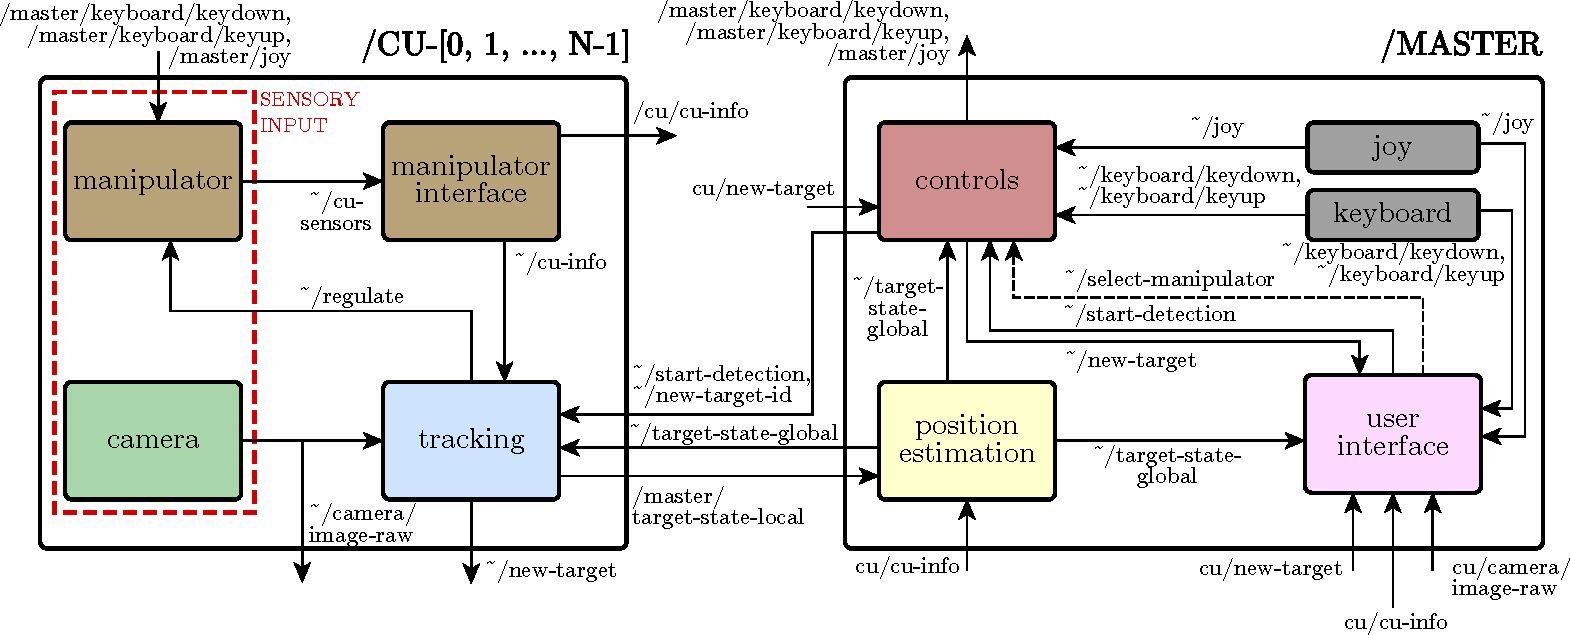
\includegraphics[width=14.5cm]{fig/sw_ols.pdf}
	\caption{The diagram of the software components represented by the ROS nodes. The communication among topics is implemented using ROS topics (normal arrows) and ROS services (dashed arrows).}
	\label{fig:sw_ols}
\end{figure}

The nodes running within the \texttt{master} namespace serve the purpose of the access point for an user (an operator) as well as the main controller of the whole system. The node \texttt{controls} keeps the information about the tracked targets and distributes the workload to the separate camera units based on their position and orientation with regards to the newly discovered target. The node \texttt{position\_estimation} calculates the triangulation and estimates the 3D position of the target. The node \texttt{GUI} implements the graphical user interface allowing the operator to control the system and the nodes \texttt{joy} and \texttt{keyboard} process the events from peripherals.

Each of the namespaces \texttt{camera\_unit\_N} controls a separate camera unit. The namespace contains the standard node \texttt{avt\_vimba\_camera} processing the input image stream from Prosilica camera and it implements the node \texttt{manipulator}, which controls the manipulator and publishes its state, and the node \texttt{detection\_and\_tracking}, which performs the computationally most expensive tasks of the object detection, learning its appearance and tracking.


%-------------------------------------------------------------------------
%-------------------------------------------------------------------------
\section{Application of Gazebo} \label{txt:application_of_gazebo}

Gazebo\footnote{The official website of Gazebo: \url{http://gazebosim.org}} is a physical simulator developed by the OSRF\footnote{Open Source Robotic Foundation: \url{http://www.osrfoundation.org/}} providing the tools to model and simulate robots in both indoor and outdoor environment. The simulator has been developed since 2002 and today represents a mature system with wide penetration and support, while being distributed as open source and freeware. 

Since the Gazebo is distributed also as one of the standard packages of the ROS framework it is straightforward to integrate the simulation environment with the already implemented ROS nodes. There are multiple advantages of using the simulator over a development using a real hardware, the main motivations were as follows:

\paragraph{testing a tracker} The Gazebo provides the ROS plugin simulating an RGB camera, which captures the virtual scene and publishes a stream of rendered images. Thus it can be used to test an object tracking algorithm using arbitrarily complex environment and moving objects (see Figure \ref{fig:gazebo_camera_stream}).

%% The screenshot of Gazebo scene and image streams from cameras.
\begin{figure}[htb]
	\centering
	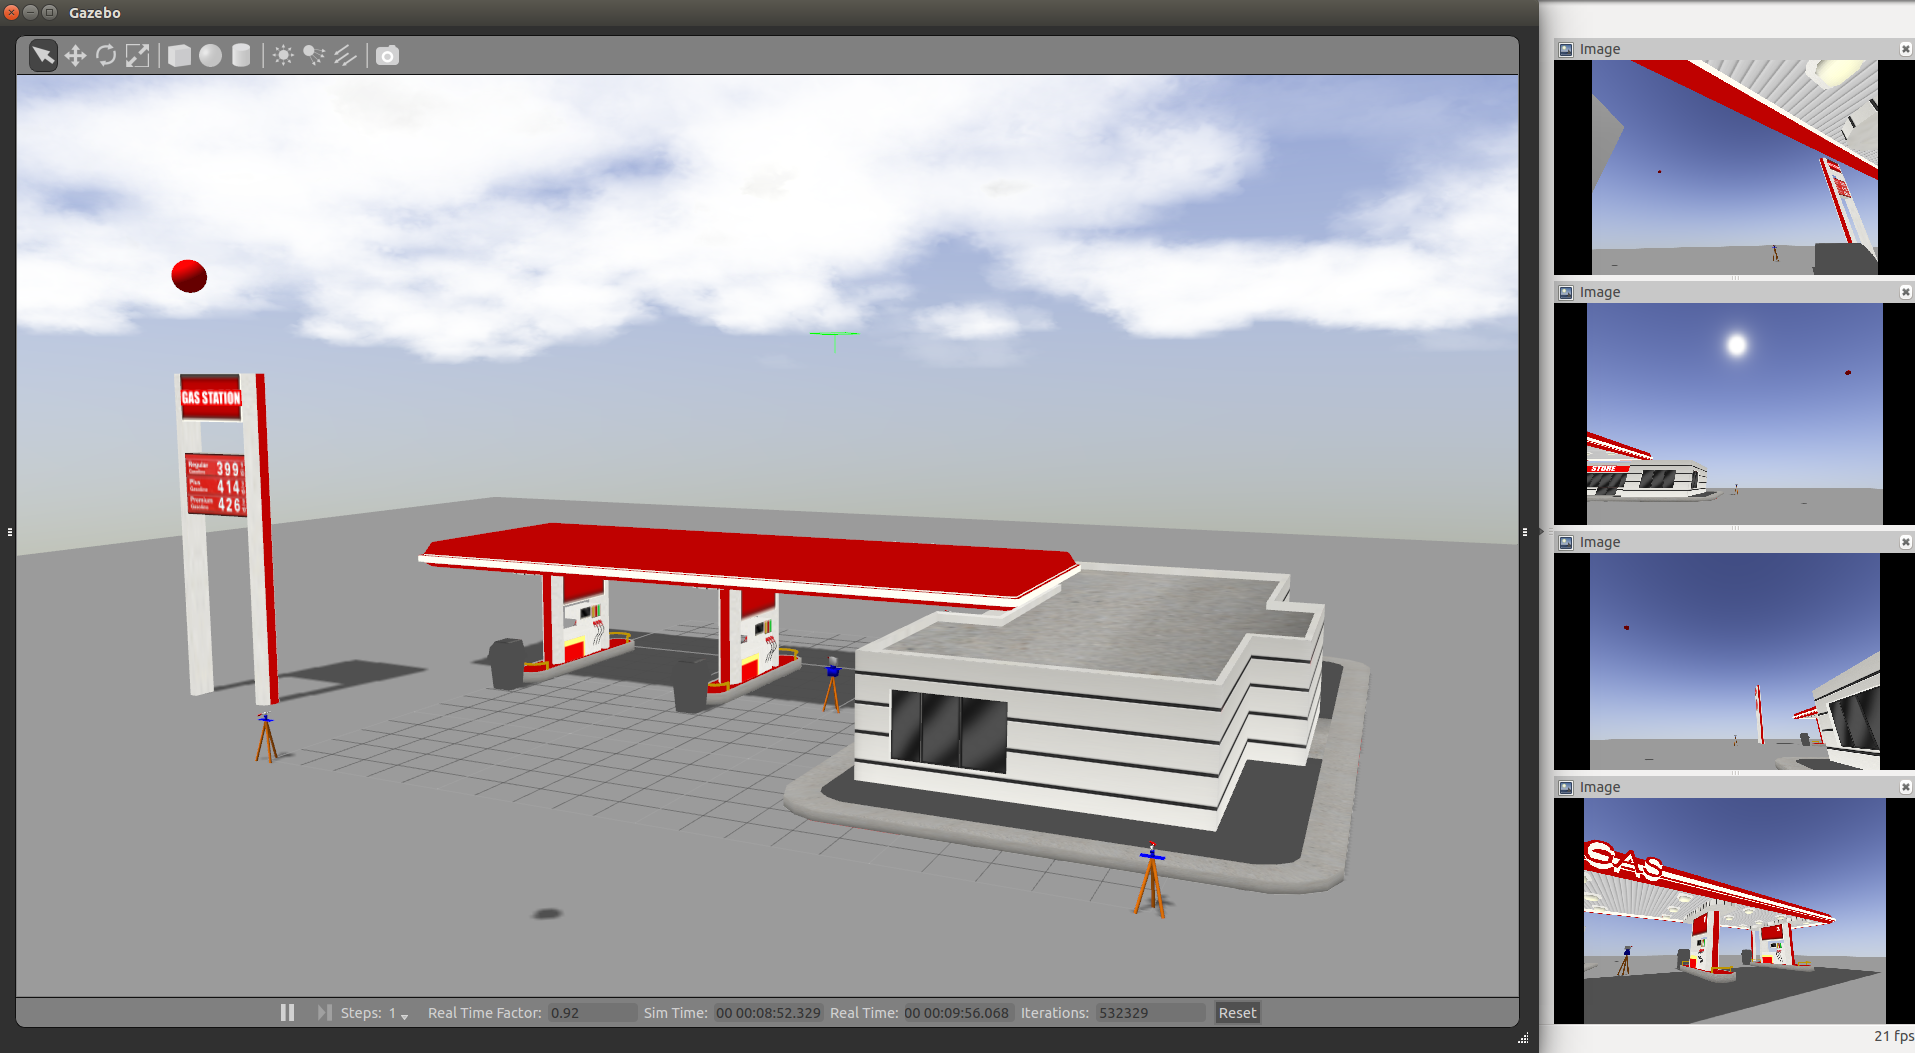
\includegraphics[width=14.5cm]{fig/gazebo_camera_stream.png}
	\caption{The screenshot of a Gazebo simulation (left) consisting of a virtual environment (the gas station), a flying object (the red sphere) and four manipulators. All four virtual camera streams are displayed real-time using \texttt{rviz} tool (right).}
	\label{fig:gazebo_camera_stream}
\end{figure}

\paragraph{testing a manipulator} It is a good practice to include a real hardware in the simulation during the development \cite{on_hw_in_the_loop}. Both actuators and sensors would be difficult to simulate properly, moreover a real manipulator is constrained in terms of the operational range (see Section \ref{txt:camera_unit}), maximum acceleration and speed and communication throughput so it is necessary to thoroughly test its performance. This so called hardware-in-the-loop simulation reveals whether the implementation of motion control is correct and whether the possibilities of the manipulator suffice to track arbitrarily fast (simulated) objects.

\paragraph{testing a triangulation} Thanks to the Gazebo it is possible to simulate a flying object with a-priory set trajectory and evaluate the precision of a position estimation algorithm using comparison between the estimated target position and a ground-truth.

%-------------------------------------------------------------------------
%-------------------------------------------------------------------------
\section{External Libraries} \label{txt:external_libraries}

Besides the framework ROS a few other publicly available libraries are used within the implementation.

\paragraph{OpenCV} Open Source Computer Vision Library\footnote{The official website of OpenCV: \url{http://opencv.org}} is a free open source library providing algorithms for image processing, computer vision and machine learning. Version 2.4.11 is used as it is a component of ROS Indigo.

\paragraph{Eigen} This open source C++ template library\footnote{The official website of Eigen: \url{http://eigen.tuxfamily.org}} implements the data structures and methods for fast and convenient solving of linear algebra problems.

\paragraph{OpenTLD} The OpenTLD library\footnote{The official website of OpenTLD: \url{http://www.gnebehay.com/tld}} represents an open source C++ implementation the TLD tracking algorithm (see Section \ref{txt:detection_and_tracking}).	

\paragraph{Serial} A cross-platform library Serial\footnote{The official website of Serial: \url{https://github.com/wjwwood/serial}} implemented in C++ provides the API for interfacing with RS-232 serial like ports. It is used to control the manipulator.

%=========================================================================
%=========================================================================
\chapter{Experiemtnal Results}

\vata[28]

%=========================================================================
%=========================================================================
\chapter{Conclusion} \label{txt:conclusion}
% 1 - 2 ns

This work presents a novel system for autonomous optical localization of aerial targets. The principle of triangulation is well known and widely used, however the main contribution of the system is the fact it is designed to operate autonomously from detecting the object to estimating its position. As the first step, a suitable placement of available camera units had to be designed and the proper hardware components, which each camera station consists of, had to be selected. A model of the camera unit represented by a kinematic chain was proposed and all camera units were then rectified in order to minimize the difference between the model and the real construction of the camera units.

As fo the software solution, the most promising computer vision techniques for both detection and tracing of the target were proposed and one of them, a free implementation of the TLD algorithm was eventually integrated in the system. The architecture of the system based on the ROS framework was designed and implemented and the physical simulation software Gazebo was used to experiment with the system placed in a virtual scene.

As far as the further development is concerned, the autonomous detection algorithm will be implemented and the tracking algorithm will be improved on since the OLS system expects a static background (as opposed to the TLD) so the background modeling could be incorporated to further improve the tracker performance. The subsystem for target handoff among the cameras will be designed and implemented and the localization algorithm will be improved on to reflect the uncertainty of the locations and orientations of the separate joints in the kinematic models and to provide the result in global geographical coordinates (most likely UTM). A proper dataset will be acquired and the system will be tested thoroughly.

\vata[5]